\documentclass[letterpaper,11pt,oneside,reqno]{amsart}
\usepackage[T2A]{fontenc}
\usepackage[utf8]{inputenc}
\usepackage[english]{babel}
\usepackage{amsmath,amssymb,amsthm,amsfonts,upgreek}
\usepackage{hyperref}
\usepackage{cleveref}
\usepackage{enumerate}
\usepackage{graphicx}
\usepackage[mathscr]{euscript}
\usepackage{color,tikz}
\usepackage[DIV15]{typearea}
% \usepackage[width=.75\textwidth]{caption}
\allowdisplaybreaks
\numberwithin{equation}{section}
\usepackage{listings}

\synctex=1
\newcommand{\note}[1]{\textsc{\color{blue}(#1)}}
\newcounter{lecture}
\newcommand{\lect}[1]{\bigskip\addtocounter{lecture}{1}\noindent{\Large{\color{red}\bf{}Lecture \#\arabic{lecture} on #1 \hrulefill}}}
% \newcommand{\lect}[1]{}
% \usepackage{refcheck}

%%%%%%%%%%%%%%%%%%%%%%%%%%%%%%%%%%%%%%%%%%%%%%%%%%%%%%%%%%%%
\newcommand{\SC}{\mathsf{SC}}
\DeclareMathOperator{\EE}{\mathbb{E}}
\DeclareMathOperator{\VAR}{\mathrm{Var}}
\DeclareMathOperator{\PP}{\mathbb{P}}
\newcommand{\Det}{\mathop{\mathrm{det}}\limits}

 
%%%%%%%%%%%%%%%%%%%%%%%%%%%%%%%%%%%%%%%%%%%%%%%%%%%%%%%%%%%%
\newtheorem{proposition}{Proposition}[section]
\newtheorem{lemma}[proposition]{Lemma}
\newtheorem{corollary}[proposition]{Corollary}
\newtheorem{theorem}[proposition]{Theorem}
\theoremstyle{definition}
\newtheorem{definition}[proposition]{Definition}
\newtheorem{remark}[proposition]{Remark}
\newtheorem{example}[proposition]{Example}
\newtheorem{exercise}[proposition]{Exercise}
%%%%%%%%%%%%%%%%%%%%%%%%%%%%%%%%%%%%%%%%%%%%%%%%%%%%%%%%%%%%

\begin{document}

\title[Notes on random matrices]{Notes on random matrices}

\author[L. Petrov]{Leonid Petrov}
\date{\today}
\maketitle

\begin{center}
	(notes by 
	Kristin Courtney;
	Stephen Hardy;
	Bryce Terwilliger;
	Daniel Franz; \ldots)
\end{center}

\begin{abstract}
	These are notes for the MATH 8380 ``Random Matrices'' course at the
	University of Virginia in Spring 2016. The notes are constantly updated,
	and the latest version can be found at the \texttt{git} repository
	\url{https://github.com/lenis2000/RMT_Spring_2016}
\end{abstract}

\bigskip

\begin{center}
\noindent\note{before \TeX{}ing, please familiarize yourself with style suggestions at\\
\url{https://github.com/lenis2000/RMT_Spring_2016/blob/master/TeXing.md}}
\end{center}
\bigskip

\setcounter{tocdepth}{1}
\tableofcontents
\setcounter{tocdepth}{3}

\lect{1/20/2016}

\section{Introduction} % (fold)
\label{sec:introduction}

\subsection{Matrices and eigenvalues} % (fold)
\label{sub:object_of_study}

The study of random matrices as a field is a patchwork of many fields.  The
main object we study is a probability distribution on a certain subset of the
set of matrices $\mathrm{Mat}(N\times N,\mathbb R \text{ or } \mathbb C)$,
thus giving us a random matrix $A$.

\begin{definition}
An {\it eigenvalue} $\lambda$ of the matrix $A$ is a root of the polynomial
$f(\lambda)=\text{det}(A-\lambda I)$, where $I$ is the identity matrix 
(we use this notation throughout the notes).  
Equivalently, $\lambda$ is an
eigenvalue if $A$ if the matrix $A-\lambda I$ is not invertible. This second
way of defining eigenvalues in fact works even when $A$ is not a finite
size matrix, but an operator in some infinite-dimensional space.
\end{definition}

We will largely be only concerned with real eigenvalues.  That is the
eigenvalues of a real symmetric matrix over $\mathbb R$ or Hermitian over
$\mathbb C$ that is where $A^*=A$
(here and everywhere below
$A^*$ means $\overline{A^{T}}$, i.e., transposition and complex conjugation).

\begin{remark}\label{rmk:complex_eigenvalues}
	The case when eigenvalues can be complex is also studied in
	the theory of random matrices, sometimes under the keyword \emph{complex
	random matrices}. 
	This area is more modern and is actively developing now.
	See, for example, \cite{gotze2010circular} for a discussion of the law of 
	large numbers.
\end{remark}

\begin{proposition}
Every eigenvalue of a Hermitian matrix is real.
\end{proposition}
\begin{proof}
Let $A$ be a Hermitian matrix, so that $A^*=A$.
Let $\lambda$ be an eigenvalue of $A$.  Let $v$ be a nonzero vector in the null
space of $A-\lambda I$.  Let $a=\overline{ v^{T}}v=|v|^2$, so
that $a$ is a positive real number.  Let $b=\overline{ v^{T}}A
v$.  Then $\bar b=\overline{ b^{T}}=\overline{\overline{
v^{T}}Av}^{T}=\overline{
v^{T}}\bar A^{T} v=\overline{
v^{T}}Av=b$, so $b$ is real.  Since $b=\lambda a$, $\lambda$
must be real. 
\end{proof}

Let $\mathcal H_N$ be the set of $N\times N$ Hermitian matrices.  For each
$N$, let $\mu_N$ be a probability measure on $\mathcal H_N$ (it can be
supported not by  the whole $\mathcal H_N$, but by a subset of it, too).  Then
for each matrix $A\in \mathcal H_N$ we may order the real eigenvalues
$\lambda_1\geq \cdots \geq \lambda_N$ of $A$ (the collection of eigenvalues
is called the \emph{spectrum} of $A$).

A collection of probability measures $\mu_N$ on $\mathcal H_N$ for each
$N\ge1$ is said to be a \emph{random matrix ensemble}. For such an ensemble,
the eigenvalues $\lambda_1^{(N)}\geq \cdots \geq \lambda_N^{(N)}$ of matrices
$N$ form random point configurations on $\mathbb{R}$ with growing numbers of points.
Our main goal is to study the asymptotic properties of these collections of points on $\mathbb{R}$,
as $N\to\infty$.

% subsection object_of_study (end)

\subsection{Why study random matrices?} % (fold)
\label{sub:why_study_random_matrices_}

Let us briefly discuss five possible motivations to study random matrices and asymptotic distributions of 
random matrix spectra.

\subsubsection{}

Matrices are a natural generalization of real numbers, so studying them would
seem natural from a  pure probability point of view. However, the development
of the theory of Random Matrices was much application driven.

\subsubsection{Hurwitz and theory of invariants} 

A. Hurwitz in the 1890s \cite{Hurwitz1897} computed the volume of orthogonal
and unitary groups of matrices.\footnote{The group $O(N)$
of orthogonal $N\times N$ matrices consists of matrices $O$ with real entries, 
for which $O^{T}O=OO^{T}=I$.
The group $U(N)$ of unitary 
$N\times N$ matrices consists of matrices $U$ with complex entries, 
for which $UU^{T}=U^{T}U=I$.
Both groups are \emph{compact}, and so possess finite Haar measures,
i.e., measures $\mu$ which are invariant under left and right shifts on the group.} 
For example, $U(1)$, the set of unitary
$1\times 1$ unitary matrices --- the unit circle --- has volume $2\pi$.  For general $N$, the
volume of $U(N)$ is the normalization constant $Z_N=\int_{U(N)} 1\cdot d(\mathrm{Haar}_N)$ in probabilistic integrals
over the Haar measure on the unitary group,
\begin{align*}
  	Z_N=2^{N(N+1)/2}\prod_{k=1}^{N}\frac{\pi^{k}}{\Gamma(k)}=2^{N(N+1)/2}\prod_{k=1}^{N}\frac{\pi^{k}}{(k-1)!}.
\end{align*}
See
\cite{diaconis2015hurwitz} for a recent survey.

\subsubsection{Statistics} 

J. Wishart in 1928 \cite{wishart1928generalised} considered random covariance matrices of 
vector-valued data. For testing the hypothesis of independence of components of the vector,
it is natural to study the distribution of the random covariance matrix 
of the uncorrelated vector (the null-hypothesis distribution). Let us assume that the components
of the vector are identically distributed.

This latter matrix ensemble (called the \emph{Wishart ensemble})
can be constructed by taking a rectangular matrix $Y$ with independent (or uncorrelated) 
identically distributed entries, and taking $A=Y^{T}Y$. Then $A$ is a square matrix
which is said to have the (\emph{real}) \emph{Wishart distribution}. 

For the purposes of statistics, the distribution of the Wishart matrix $A$ should be 
compared with the distribution under the alternate hypothesis that the entries of the vector are correlated.
For certain assumed nature of the correlation structure, this leads to
considering \emph{spiked random matrices} of the form $A+R$, where $A$
is Wishart and $R$ is a finite-rank perturbation. It turns out that sometimes the 
presence of a nonzero matrix $R$ may be detected by looking at the spectrum of $A+R$,
which again leads to considering spectra of random matrices.
One reference (among many others which are not mentioned) 
relevant for the current research on spiked random matrices is
\cite{BBR2005phase}.

\subsubsection{Nuclear physics} 

Active development of the theory of random matrices begins in the 1950s when
Wigner, Dyson, Mehta, and their collaborators explored nuclear physics
applications.  In nuclear quantum physics a state of a system is an operator
on an $L^2$ space of functions; its eigenvalues are the energy levels of the
system.  For  large nuclei it is difficult to analyze the operator in $L^2$
directly, but Wigner postulated that differences in energy levels could be
modeled by differences in eigenvalues of certain classes of matrices under
appropriate probability measures. That is, the collections $\{\Delta E_i\}$
and $\{\lambda_i-\lambda_{i+1}\}$ should be statistically close. Moreover, the
random matrix ensemble should have the same symmetry as that quantum system.
The symmetry classes of random matrices are discussed in detail in a recent
survey \cite{Zirnbauer2010}. Dyson proposed a model of stochastic dynamics of
energies (eigenvalues of random matrices). We will study the Dyson's Brownian
motion later. 

Section 1.1 of the book \cite{mehta2004random} contains a nice outline of 
physical applications of random matrices.

\subsubsection{Number theory} 

Dyson and Montgomery uncovered number theoretic applications of random matrices 
in the 1970's \cite{montgomery1973pair}, with Odlyzko in the 1980's \cite{odlyzko1987distribution} providing powerful numerical simulations.

Consider the Riemann Zeta Function
\begin{equation*}
\zeta(s)=\sum_{n=1}^{\infty}\frac{1}{n^s} \qquad \text{ for } s\in \mathbb C \text{ with the real part of } s>1
\end{equation*}

Riemann showed that $\zeta(s)$ can be analytically continued to a function on
$\mathbb C$ with a pole at $s=1$.  The famous Riemann hypothesis is that all
the zeroes of the Zeta function with real part greater than 0 lie on the
\emph{critical line} $\frac{1}2+i t$.  It turns out that the distribution of
the zeroes on the critical line can be linked to the distribution of
eigenvalues of random matrices.  Consider the zeros $\frac12+it_n$ of the zeta function
with $t_n\in\mathbb{R}$. Let us define
\begin{equation*}
w_n=\frac{t_n}{2\pi}\log\left(\frac{|t_n|}{2\pi}\right),
\end{equation*}
then $\displaystyle \lim_{L\to\infty} \frac{1}{L} \#\left\{w_n\in [0,L]\right\}=1$, i.e., the 
average density of the $w_n$'s is $1$.
The theorem/conjecture of Montgomery\footnote{Depending in part
on the Riemann hypothesis and in part on 
how strong is the assumed convergence in \eqref{Montgomery_zeta}.} states that the pair correlations of the 
zeroes of the zeta function have the form
\begin{equation}\label{Montgomery_zeta}
	\lim_{L\to\infty} \frac{1}{L}\# \left\{\begin{array}{c} w_n\in [0,L] \\ \alpha\leq w_n-w_m\leq \beta \end{array}\right\} 
	\sim \int_\alpha^\beta \left(\delta(x)+1 -\frac{\sin^2(\pi x)}{\pi^2 x^2}\right)\, dx,
\end{equation}
where $\delta(x)$ is the Dirac delta.
Further details on this and other connections
between number theory and random matrices
can be found in \cite{keating2000random}, \cite{keating2006random}.

\begin{remark}
	There are accounts of Montgomery 
	meeting Dyson at teatime at the IAS; the latter pointed
	out the connection between Montgomery's formula and the eigenvalue
	distributions of random matrices. 
	A quick Internet search lead to the following links containing details:
	\url{https://www.ias.edu/articles/hugh-montgomery} and
	\url{http://empslocal.ex.ac.uk/people/staff/mrwatkin//zeta/dyson.htm}.
\end{remark}


% subsection why_study_random_matrices_ (end)

\subsection{Course outline} % (fold)
\label{sub:goals_for_the_course}

The course will consist of five main parts, with the last part being optional:

\begin{enumerate}[\bf1.]
	\item Limit shape results for random matrices (such as Wigner's Semicircle Law). Connections to Free Probability.
	\item Concrete ensembles of random matrices (GUE, circular, and Beta ensembles). Bulk and edge asymptotics via exact computations. Connection to determinantal point processes.
	\item Dyson's Brownian Motion and related stochastic calculus.
	\item Universality of random matrix asymptotics.
	\item (optional, depending on time available) Discrete analogues of random matrix models: random permutations, random tilings, interacting particle systems.
\end{enumerate}

% subsection goals_for_the_course (end)

% section introduction (end)

\section{Wigner's Semicircle Law and its combinatorial proof} % (fold)
\label{sec:wigner_s_semicircle_law}

After discussing the object and motivations for studying random matrices, let
us proceed to the first part of the course --- the laws of large numbers
for the eigenvalue distributions of random matrices. 
The first of these laws of large numbers is the 
\emph{Wigner's Semicircle Law}. It dates back to 
\cite{wigner1955characteristic}.

\subsection{Real Wigner matrices} % (fold)
\label{sub:real_wigner_matrices}

A particular ensemble of random matrices is the \emph{real Wigner matrices}.
Let $A\in \mathrm{Mat}(N\times N,\mathbb R)$ with $A=(a_{ij})_{i,j=1}^N$ such
that $a_{ij}=a_{ji}$. To describe the distribution of the random matrix $A$ we only need to
describe the upper triangular portion of $A$.

\begin{definition}\label{def:real_Wigner}
The law of the real Wigner $N\times N$ matrix is described as follows:
\begin{itemize}
	\item $\{a_{ij}\}_{i\leq j}$ is an independent collection of random variables
	\item $\{a_{ii}\}_{i=1}^N$ is iid\footnote{Independent identically
	distributed.}, and $\{a_{ij}\}_{i<j}$ is iid.
	\item $\EE a_{ij}=0$ for all $i,j$; $\EE a_{ij}^2=2$ for $i=j$; and $\EE a_{ij}^2=1$ for $i\neq j$.
	\item all moments of $a_{ij}$ are finite.
\end{itemize}
The last condition greatly simplifies technicalities of the proofs,
but most results on real Wigner matrices hold under weaker assumptions.
\end{definition}

\begin{example}
A large class of Wigner random matrices
(which helps justify why in $A$ the variances on the diagonal must be twice the 
off-diagonal
variances) can be constructed as follows.
Suppose the collection of random variables $x_{ij}$ for $1\leq i,j\leq N$ is iid with $\EE x_{ij}=0$ and $\EE x_{ij}^2=1$.  Let $X=(x_{ij})$ be an $N\times N$ matrix.  Define
\begin{equation*}
	A:=\frac{X+X^T}{\sqrt{2}}.
\end{equation*}
One readily sees that $A$ is real Wigner. Namely, for example,
$a_{11}=\frac{x_{11}+x_{11}}{\sqrt 2}=\sqrt 2 x_{11}$, so $\EE a_{11}=0$ 
and $\EE a_{11}^2=2\EE x_{11}^2=2$.  If $N\geq 2$ then $a_{12}=a_{21}$ with $a_{12}=\frac{x_{12}+x_{21}}{\sqrt 2}$, 
and we have $\EE a_{12}=0$ and $\VAR a_{12}=\frac{1}{2}\VAR(x_{12}+x_{21})=1$ because $x_{12}$ and $x_{21}$ are independent.
\end{example}

% subsection real_wigner_matrices (end)

\subsection{Gaussian Orthogonal Ensemble} % (fold)
\label{sub:gaussian_orthogonal_ensemble}

A special case of real Wigner matrices  is when each $a_{ij}$ is Gaussian.
This case is called the \emph{Gaussian Orthogonal Ensemble} (\emph{GOE}).

\begin{lemma}
	The distribution of the GOE is orthogonally invariant, that is,
	if $A$ has the GOE distribution and $O\in O(N)$ is a fixed
	orthogonal matrix, then $OAO^{T}$ has the same probability distribution~as~$A$.
\end{lemma}
\begin{proof}
	It is not hard to check that the
	probability density of $A$ with respect to the 
	Lebesgue measure on $\mathrm{Mat}(N\times N,\mathbb R)$
	(this space is isomorphic to $\mathbb{R}^{N(N+1)/2}$
	by considering the upper triangular part)
	has the form
	\begin{align*}
		f(A)=c \exp(-\mathop{\mathrm{tr}}(A^2)),
	\end{align*}
	where $c$ is a normalization constant.\footnote{Here 
	and below $\mathop{\mathrm{tr}}(A)=a_{11}+a_{22}+\ldots+a_{NN}$ 
	is the trace of a matrix.}  Since the matrix trace
	is invariant under cyclical permutations, 
	\begin{align*}
		\mathop{\mathrm{tr}}(OA^2O^{T})
		=\mathop{\mathrm{tr}}(A^2O^{T}O)
		=\mathop{\mathrm{tr}}(A^2).
	\end{align*}
	Thus, $OA^2O^{T}\stackrel{\mathcal D}{=} A$.
\end{proof}

We will discuss the GOE (and its close relative GUE, Gaussian Unitary Ensemble)
in detail in the course later, but for now we will focus on 
properties of real Wigner matrices with general entry distribution.

% subsection gaussian_orthogonal_ensemble (end)

\subsection{Formulation of the Wigner Semicircle Law} % (fold)
\label{sub:formulation_of_the_wigner_semicircle_law}

For a real Wigner matrix $A_N\in\mathrm{Mat}(N\times N)$ let
$\lambda_1^{(N)}\geq \cdots \geq \lambda_N^{(N)}$ be the eigenvalues of $A_N$.
The \emph{empirical distribution of the eigenvalues} is
\begin{equation}\label{EmpiricalDistributionOfEigenvalues}
	L_N=\frac{1}{N}\sum_{i=1}^N \delta_{N^{-1/2}\lambda_{i}^{(N)}}.
\end{equation}
That is, we put delta masses of size $1/N$ into the
$N$ positions of rescaled eigenvalues 
$\lambda_{i}^{(N)}/\sqrt N$. This rescaling will turn out to be appropriate for the 
law of large numbers.
Note that $L_N$ is a probability measure on $\mathbb{R}$.

\begin{remark}
	For the purposes of asymptotic statements, we will always assume that the 
	off-diagonal entries of real Wigner matrices 
	$A=A_N$ have the same fixed distribution independent of $N$,
	and similarly the diagonal entries 
	have the same fixed (but different) distribution.
\end{remark}

\begin{figure}[htbp]
	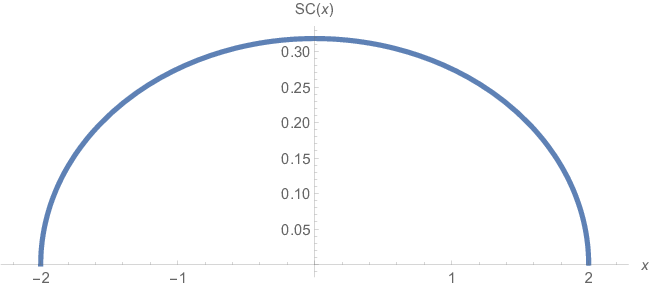
\includegraphics[width=.5\textwidth]{img/SC.png}
	\caption{Semicircle density $\SC(x)$.}
	\label{fig:semicircle}
\end{figure}

\begin{figure}[htbp]
	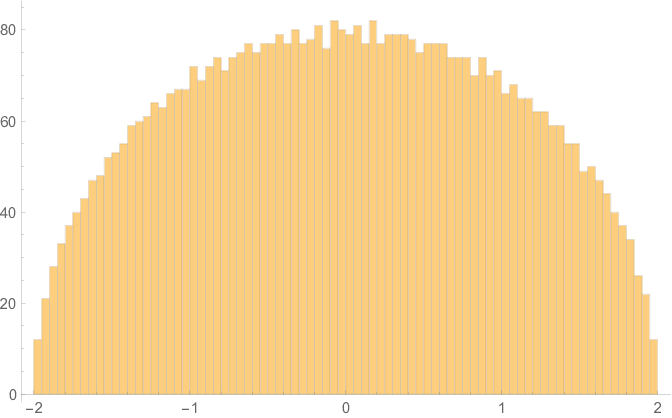
\includegraphics[width=.5\textwidth]{img/Wigner1.png}
	\caption{Histogram of the empirical distribution 
	$L_N$ for $N=5000$.}
	\label{fig:Wigner}
\end{figure}

\begin{definition}
	The semicircle distribution $\SC$ is 
	a fixed probability distribution on $\mathbb{R}$
	supported on $[-2,2]$
	which is absolutely continuous with respect to the
	Lebesgue measure and has the density
	\begin{equation}\label{SemicircleDistribution}
		\SC(x):=\frac{1}{2\pi}\sqrt{4-x^2}, \qquad -2\leq x\leq 2.
	\end{equation}
	See \Cref{fig:semicircle}.

	Note that slightly abusing the notation, by $\SC$ we will denote both the
	semicircle distribution and its probability density \eqref{SemicircleDistribution}.
\end{definition}

\begin{theorem}[Wigner's Semicircle Law]\label{thm:SemicircleLaw}
	As $N\to\infty$,
	the empirical distributions 
	$L_N$ converge weakly, in probability to the 
	semicircle distribution $\SC$.
\end{theorem}

Let us explain what we mean by convergence ``weakly in probability''. Formally this means that
for any bounded continuous function $f$ on $\mathbb R$ ($f\in C_B(\mathbb R)$) and each $\varepsilon>0$ we have 
\begin{equation}\label{WignerSemicircleLaw}
\lim_{N\to\infty}\mathbb P\left(\left|\int_{\mathbb R} f\,dL_N-\int_{\mathbb R} f\,d\SC\right|>\varepsilon\right)=0.
\end{equation}
That is, ``in probability'' means the usual convergence in probability  of
random elements $L_N$ to a (nonrandom) element $\SC$.  On the other hand,
``weakly'' specifies the metric on the space of probability measures on
$\mathbb{R}$ (to which all $L_N$ and $\SC$ belong). Convergence of probability
measures in this metric simply means weak convergence of probability measures
on $\mathbb{R}$.

In other words,
let us use a convenient notation for the pairing $\langle f,\mu\rangle
=\int_{\mathbb R} f\,d\mu=\int_{\mathbb R}f(x)\,\mu(dx)$ for a given
function $f$ and measure $\mu$.  If $\mu$ is a random measure (such as $L_N$,
since $L_N$ depends on $A_N$ which is random), then $\langle f,\mu\rangle$ is
a random element of $\mathbb R$ (usually we say random variable).  Since $\SC$
is not random, the pairing $\langle f,\SC\rangle$ is a fixed number for a given function $f$.  The
Semicircle Law thus states that for any given $f\in C_B(\mathbb R)$ the random variable
$\langle f,L_N\rangle$ converges in probability to the constant $\langle f,\SC\rangle$ which may be written as
\begin{equation}\label{WignerSemicircleLaw_langle}
\forall \varepsilon>0,\qquad \lim_{N\to\infty}\PP\left(\left|\langle f,L_N\rangle-\langle f,\SC\rangle\right|>\varepsilon\right)=0,
\end{equation}
which is the same as \eqref{WignerSemicircleLaw}.

\begin{remark}
	This type of convergence is reminiscent of the classical weak law of large numbers: for
	$\{X_i\}_{i=1}^\infty$ iid random variables with $\EE|X_1| <\infty$, the random
	variables $\dfrac{1}N\sum_{i=1}^N X_i$ converge to the constant $\EE X_1$ in probability as $N\to\infty$.
\end{remark}

% subsection formulation_of_the_wigner_semicircle_law (end)

\lect{1/25/2016}

\subsection{Strategy of the proof} % (fold)
\label{sub:strategy_of_the_proof}

We will employ the following strategy in our proof of the Wigner's semicircle
law. This is only the first of the proofs we will consider, and it is based on
the computation of moments and on the related combinatorics. Recall that for a
probability measure $\mu$ the quantities $\langle x^{k},\mu\rangle$,
$k=0,1,2,\ldots$, are called the \emph{moments} of $\mu$.

First, in \Cref{sub:moments_of_the_semicircle_distribution}
we will compute the moments  $m_k:=\langle x^k, \SC\rangle$ of the
limiting semicircle distribution, and identify the answer in terms of the
Catalan numbers. Our second step in the proof is to show the convergence
$\lim_{N\to\infty}\EE \langle x^k,L_N\rangle = m_k$ for each $k$. We do this in \Cref{sub:convergence_of_expectations_}
below.
The third
step (in \Cref{sub:variances_langle_x_k_l_nrangleto0_}) 
is to show that  the variance of $\langle x^k,L_N\rangle$ goes to zero as
$N\to\infty$ for each $k$. Finally, to complete the proof we will need to
justify that  the convergence \eqref{WignerSemicircleLaw_langle} for any
function $f(x)$ follows from the case of $f(x)=x^{k}$, $k=0,1,2,\ldots$.
This is done in \Cref{sub:completing_the_proof_WSCL}.

% subsection strategy_of_the_proof (end)

\subsection{Moments of the semicircle distribution} % (fold)
\label{sub:moments_of_the_semicircle_distribution}

Here we will compute the moments of the semicircle distribution:
\begin{equation*}
m_k=\langle x^k, \SC\rangle
=\int_{-2}^2 x^k\, \SC(x)\,dx
=\int_{-2}^2 x^k \left( \frac{\sqrt{4-x^2}}{2\pi}\right)\,dx.
\end{equation*}

Clearly, by symmetry we have $m_k=0$ for $k$ odd. If $k$ is even, let us perform a trigonometric substitution
$x=2\sin \theta$, $-\frac\pi2\le \theta\le \frac\pi2$, in the above integral:
\begin{align}\label{SC_moments_m_2k}
	m_{2k}=\frac{2^{2k+1}}{\pi}\int_{-\frac\pi2}^{\frac\pi2}\sin^{2k}\theta\cos^{2}\theta \,d\theta.
\end{align}

\begin{lemma}
	We have
	\begin{align*}
		\frac{1}{\pi}\int_{-\frac\pi2}^{\frac\pi2}\sin^{2k}\theta\, d\theta=
		\frac{(2k-1)!!}{2^k k!},
	\end{align*}
	where recall that $(2k-1)!!=1\cdot 3\cdot 5\cdots (2k-3)(2k-1)$.
\end{lemma}	
\begin{proof}
	Denote the integral in the right-hand side by $\alpha_{k}$. Observe that $\alpha_0=1$.
	Integrating by parts for $k\ge1$, we have
	\begin{align*}
		\alpha_k=
		-\frac{1}{\pi}\int_{-\frac\pi2}^{\frac\pi2}\sin^{2k-1}\theta\, d(\cos\theta)
		=\frac{1}{\pi}\int_{-\frac\pi2}^{\frac\pi2}
		(2k-1)\sin^{2k-2}\theta\cos^{2}\theta\, d\theta
		=(2k-1)\alpha_{k-1}-(2k-1)\alpha_{k}.
	\end{align*}
	Therefore, the quantities $\alpha_k$ satisfy
	\begin{align*}
		\frac{\alpha_k}{\alpha_{k-1}}=\frac{2k-1}{2k},
	\end{align*}
	which is the same relation as for the quantities 
	$\frac{(2k-1)!!}{2^k k!}$.
	This completes the proof.		
\end{proof}
By relating $m_{2k}$ \eqref{SC_moments_m_2k} and $\alpha_k$ in the above lemma,
we see that the even moments of the semicircle distribution are given by 
\begin{align}\label{m_2k_Catalan}
	m_{2k}=\frac{1}{k+1}\binom{2k}{k},\qquad k=0,1,2,\ldots.
\end{align}
These quantities are called the \emph{Catalan numbers}.

% subsection moments_of_the_semicircle_distribution (end)

\subsection{Catalan numbers} % (fold)
\label{sub:catalan_numbers}

The Catalan numbers $\mathrm{Cat}_k$ are defined as
\begin{align}\label{Catalan_def}
	\mathrm{Cat}_k:=\frac{1}{k+1}\binom{2k}{k},\qquad
	k=0,1,2,\ldots.
\end{align}
The first twenty one of them are
\begin{align*}
	1,1,2,5,14,42,132,429,1430,4862,16796,58786,208012,742900,2674440,\\9694845,35357670,129644790,477638700,1767263190,6564120420.
\end{align*}
They are ubiquitous in combinatorics: for
example, there are more than 200 families of objects  enumerated by the
Catalan numbers \cite{stanley2015catalan}. A list of references and
properties of Catalan numbers may be found at \cite{CatalanOEIS}.

Here we will list a number of properties of the Catalan numbers which will be important 
for our proof of the semicircle law.

\subsubsection{Dyck paths} % (fold)
\label{ssub:dyck_paths}

\begin{definition}
	A \emph{Dyck path} of length $2n$ is a 
	sequence $d_0,d_1,\ldots,d_{2n}$ such that
	$d_0=d_{2n}=0$, $d_{i+1}-d_{i}=\pm1$ for all $i$,
	and that $d_i\ge0$ for all $i$. Graphically Dyck paths can be represented as 
	in \Cref{fig:Dyck}.
\end{definition}

\begin{figure}[htbp]
	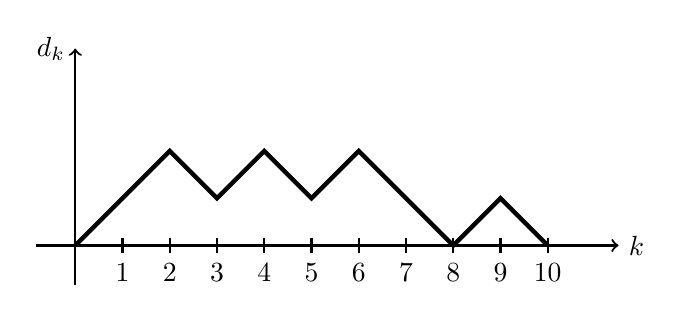
\begin{tikzpicture}[scale=1,thick]
		\draw[->] (-.5,0)--++(7.4,0) node [right] {$k$};
		\draw[->] (0,-.5)--++(0,3) node [left] {$d_k$};
		\foreach \ii in {1,...,10}
		{
			\draw (\ii*.6,.1)--++(0,-.2) node [below] {$\ii$};
		}
		\draw[ultra thick] (0,0)--++(.6,.6)--++(.6,.6)
		--++(.6,-.6)--++(.6,.6)--++(.6,-.6)
		--++(.6,.6)--++(.6,-.6)--++(.6,-.6)--++(.6,.6)--++(.6,-.6);
	\end{tikzpicture}
	\caption{A Dyck path of length $2n=10$.}
	\label{fig:Dyck}
\end{figure}

\begin{figure}[htbp]
	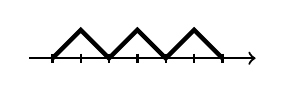
\begin{tikzpicture}[scale=.6,thick]
		\draw[->] (-.5,0)--++(4.8,0);
		\foreach \ii in {0,...,6}
		{
			\draw (\ii*.6,.1)--++(0,-.2);
		}
		\draw[ultra thick] 
		(0,0)--++(.6,.6)--++(.6,-.6)
		--++(.6,.6)--++(.6,-.6)--++(.6,.6)
		--++(.6,-.6);
	\end{tikzpicture}
	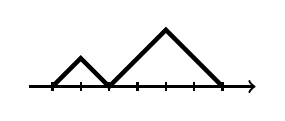
\begin{tikzpicture}[scale=.6,thick]
		\draw[->] (-.5,0)--++(4.8,0);
		\foreach \ii in {0,...,6}
		{
			\draw (\ii*.6,.1)--++(0,-.2);
		}
		\draw[ultra thick] 
		(0,0)--++(.6,.6)--++(.6,-.6)
		--++(.6,.6)--++(.6,.6)--++(.6,-.6)
		--++(.6,-.6);
	\end{tikzpicture}
	
	\rule{0pt}{34pt}
	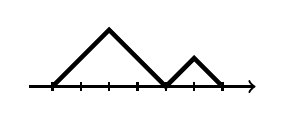
\begin{tikzpicture}[scale=.6,thick]
		\draw[->] (-.5,0)--++(4.8,0);
		\foreach \ii in {0,...,6}
		{
			\draw (\ii*.6,.1)--++(0,-.2);
		}
		\draw[ultra thick] 
		(0,0)--++(.6,.6)--++(.6,.6)
		--++(.6,-.6)--++(.6,-.6)--++(.6,.6)
		--++(.6,-.6);
	\end{tikzpicture}

	\rule{0pt}{41pt}
	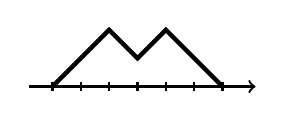
\begin{tikzpicture}[scale=.6,thick]
		\draw[->] (-.5,0)--++(4.8,0);
		\foreach \ii in {0,...,6}
		{
			\draw (\ii*.6,.1)--++(0,-.2);
		}
		\draw[ultra thick] 
		(0,0)--++(.6,.6)--++(.6,.6)
		--++(.6,-.6)--++(.6,.6)--++(.6,-.6)
		--++(.6,-.6);
	\end{tikzpicture}
	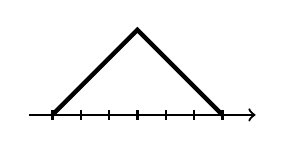
\begin{tikzpicture}[scale=.6,thick]
		\draw[->] (-.5,0)--++(4.8,0);
		\foreach \ii in {0,...,6}
		{
			\draw (\ii*.6,.1)--++(0,-.2);
		}
		\draw[ultra thick] 
		(0,0)--++(.6,.6)--++(.6,.6)
		--++(.6,.6)--++(.6,-.6)--++(.6,-.6)
		--++(.6,-.6);
	\end{tikzpicture}
	\caption{All five Dyck paths of length $2n=6$.
	The first two paths first return to zero at time $2j=2$, the 
	third path first returns to zero at time $2j=4$,
	and the last two paths first return to zero at time $2j=6$.}
	\label{fig:Dyck3}
\end{figure}

\begin{exercise}\label{exec:Dyck_Catalan}
	The number of Dyck paths of length $2n$ is equal to the Catalan number $\mathrm{Cat}_n$.
\end{exercise}
\begin{proof}[Idea]
	Use the \emph{reflection principle} --- a tool used in 
	the study of random walks and Brownian motion. 
	See \url{https://en.wikipedia.org/wiki/Catalan_number#Second_proof} for details.

	Another way to count the Dyck paths is to first establish the recurrence \eqref{Catalan_recurrence}, and then use generating
	functions to solve the recurrence (see \Cref{rmk:from_recurrence_to_explicit_formula} below).
\end{proof}

% subsubsection dyck_paths (end)

\subsubsection{Recurrence} % (fold)
\label{ssub:recurrence}

\begin{lemma}\label{lemma:Dyck_and_recurrence}
The Catalan numbers satisfy the recurrence relation
\begin{align}\label{Catalan_recurrence}
	\mathrm{Cat}_0=1,\qquad
	\mathrm{Cat}_{n}=\sum_{j=0}^n \mathrm{Cat}_{j-1}\mathrm{Cat}_{n-j}.
\end{align}
\end{lemma}
\begin{proof}
	The easiest way to see this is by counting the Dyck paths: let the first time a Dyck path 
	reaches $0$ be $2j$, then $j$ can be any number from $1$ to $n$ (see \Cref{fig:Dyck3}). 
	The part of the Dyck path after time $2j$ is independent from the 
	part before $2j$. The number of paths 
	from $2j$ to $2n$ is exactly $\mathrm{Cat}_{n-j}$. The 
	number of paths from $0$ to $2j$ 
	(with the condition that they do not get to $0$ in the meantime)
	can be seen to be $\mathrm{Cat}_{j-1}$ by cutting out the first up and the 
	last down steps. This implies the recurrence.
\end{proof}

\begin{remark}\label{rmk:from_recurrence_to_explicit_formula}
	The recurrence \eqref{Catalan_recurrence} provides a way to 
	get the explicit formula \eqref{Catalan_def}. Namely, considering
	the generating function $G(z)=\sum_{n=0}^{\infty}\mathrm{Cat}_n z^{n}$, 
	we see that \eqref{Catalan_recurrence} implies
	\begin{align*}
		G(z)=zG(z)^{2}+1.
	\end{align*}
	This equation on $G(z)$ has two solutions $\frac{1\pm\sqrt{1-4z}}{2z}$, 
	of which we should pick 
	$\frac{1-\sqrt{1-4z}}{2z}$ because the other solution diverges as $z\to0$.
	The Taylor expansion of this function
	is
	\begin{align*}
		\frac{1-\sqrt{1-4z}}{2z}=
		\sum_{n=0}^{\infty}\frac{1}{n+1}\binom{2n}n z^{n}=
		1+z+2 z^2+5 z^3+14 z^4+42 z^5+132 z^6+\ldots,
	\end{align*}
	which converges for $|z|<\frac14$.
	This shows that the Dyck paths are enumerated by the Catalan numbers.
\end{remark}

% subsubsection recurrence (end)

\subsubsection{Trees} % (fold)
\label{ssub:rooted_labeled_trees}

As was mentioned before, the Catalan numbers enumerate
numerous families of combinatorial objects. We will need one more family of 
such objects --- \emph{rooted ordered trees}. An ordered tree is a rooted tree (i.e., a tree with a distinguished
vertex $R$ called the \emph{root})
in which children of every vertex are linearly ordered. 
On pictures this ordering will be represented from left to right (see \Cref{fig:ordered_tree}).

\begin{figure}[htbp]
	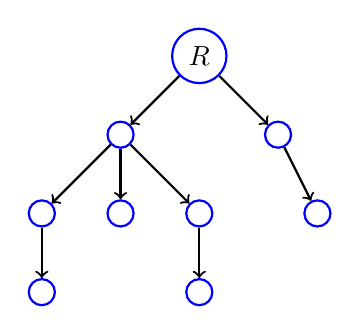
\begin{tikzpicture}[scale=1,thick,
	block/.style ={circle, draw=blue, thick ,align=center, minimum height=0.3em}]
		\node[block] (root) at (0,0) {$R$};
		\node[block] (a1) at (-1,-1) {};
		\node[block] (a2) at (1,-1) {};
		\node[block] (c1) at (1.5,-2) {};
		\node[block] (b1) at (-1,-2) {};
		\node[block] (b2) at (-2,-2) {};
		\node[block] (b3) at (0,-2) {};
		\node[block] (d1) at (0,-3) {};
		\node[block] (d2) at (-2,-3) {};
		\draw[->] (root)--(a1);
		\draw[->] (root)--(a2);
		\draw[->] (a1)--(b1);
		\draw[->] (a1)--(b2);
		\draw[->] (a1)--(b3);
		\draw[->] (a2)--(c1);
		\draw[->] (b3)--(d1);
		\draw[->] (b2)--(d2);
	\end{tikzpicture}
	\hspace{60pt}
	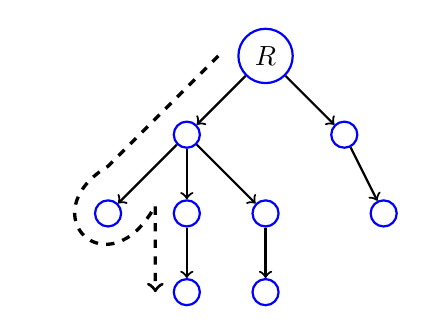
\begin{tikzpicture}[scale=1,thick,
	block/.style ={circle, draw=blue, thick ,align=center, minimum height=0.3em}]
		\node[block] (root) at (0,0) {$R$};
		\node[block] (a1) at (-1,-1) {};
		\node[block] (a2) at (1,-1) {};
		\node[block] (c1) at (1.5,-2) {};
		\node[block] (b1) at (-1,-2) {};
		\node[block] (b2) at (-2,-2) {};
		\node[block] (b3) at (0,-2) {};
		\node[block] (d1) at (0,-3) {};
		\node[block] (d2) at (-1,-3) {};
		\draw[->] (root)--(a1);
		\draw[->] (root)--(a2);
		\draw[->] (a1)--(b1);
		\draw[->] (a1)--(b2);
		\draw[->] (a1)--(b3);
		\draw[->] (a2)--(c1);
		\draw[->] (b3)--(d1);
		\draw[->] (b1)--(d2);
		\draw[->,dashed, very thick] (-.6,0)--++(-1.4,-1.4) .. controls (-3,-2) and (-2,-3) .. (-1.4,-1.9) --++ (0,-1.1);
	\end{tikzpicture}
	\caption{These trees are isomorphic as rooted trees, but are different
	as rooted ordered trees. A beginning of the walk of 
	\Cref{exec:trees_are_Catalan} is displayed for the second tree.}
	\label{fig:ordered_tree}
\end{figure}

\begin{figure}[htbp]
	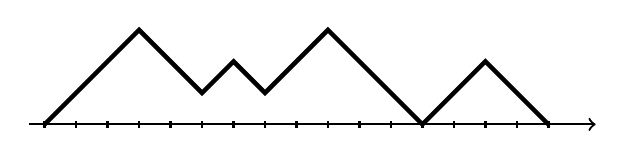
\begin{tikzpicture}[scale=.4,thick]
		\draw[->] (-.5,0)--++(18,0);
		\foreach \ii in {0,...,16}
		{
			\draw (\ii,.1)--++(0,-.2);
		}
		\draw[ultra thick] (0,0)--++(1,1)--++(1,1)--++(1,1)
		--++(1,-1)--++(1,-1)
		--++(1,1)--++(1,-1)
		--++(1,1)--++(1,1)
		--++(1,-1)--++(1,-1)--++(1,-1)
		--++(1,1)--++(1,1)
		--++(1,-1)--++(1,-1);
	\end{tikzpicture}
	\hspace{30pt}
	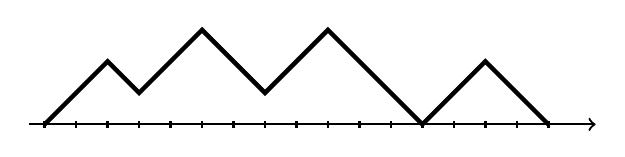
\begin{tikzpicture}[scale=.4,thick]
		\draw[->] (-.5,0)--++(18,0);
		\foreach \ii in {0,...,16}
		{
			\draw (\ii,.1)--++(0,-.2);
		}
		\draw[ultra thick] (0,0)--++(1,1)--++(1,1)--++(1,-1)
		--++(1,1)--++(1,1)
		--++(1,-1)--++(1,-1)
		--++(1,1)--++(1,1)
		--++(1,-1)--++(1,-1)--++(1,-1)
		--++(1,1)--++(1,1)
		--++(1,-1)--++(1,-1);
	\end{tikzpicture}
	\caption{Dyck paths corresponding to the rooted ordered trees in \Cref{fig:ordered_tree}
	(see \Cref{exec:trees_are_Catalan}).}
	\label{fig:ordered_tree_Dyck}
\end{figure}

\begin{lemma}\label{lemma:trees_are_Catalan}
	The number of rooted ordered trees with 
	$n+1$ vertices (including the root) is equal to the Catalan number $\mathrm{Cat}_n$.
\end{lemma}
\begin{proof}
	Assume that the leftmost subtree contains $j$ vertices (without the root), then the 
	rest of the tree including the root contains $n-j+1$ vertices. This readily implies the 
	recurrence \eqref{Catalan_recurrence}, which establishes the claim.
\end{proof}

\begin{exercise}\label{exec:trees_are_Catalan}
	By comparing the proof of \Cref{lemma:Dyck_and_recurrence,lemma:trees_are_Catalan}, 
	come up with a bijection between
	Dyck paths and ordered rooted trees.
\end{exercise}
\begin{proof}[Idea]
	Consider the walk around the tree (such that the tree is always to the left of the walker),
	which starts to the left of the root. Let $d_k$ be the distance of the walker from the root.
	The Dyck paths corresponding to trees in \Cref{fig:ordered_tree}
	are given in \Cref{fig:ordered_tree_Dyck}.
\end{proof}

% subsubsection rooted_labeled_trees (end)

% subsection catalan_numbers (end)

\subsection{Convergence of expectations $\EE \langle x^k,L_N\rangle \to m_k$} % (fold)
\label{sub:convergence_of_expectations_}

With the Catalan preparations in place, let us return to the semicircle law. 
We would like to show that 
\begin{align}\label{desired_convergence_of_averages_in_WSCL}
	\lim_{N\to\infty}\EE \langle x^k,L_N\rangle = m_k=\begin{cases}
		0,&\textnormal{$k$ odd};\\
		\mathrm{Cat}_{k/2},&\textnormal{$k$ even}.
	\end{cases}
\end{align}

First, observe that the left-hand side has the form
\begin{equation*}
\begin{split}
\EE\langle x^k,L_N\rangle&=\EE\int_{\mathbb R}x^k\,L_N(dx)\\
&=\EE\int_{\mathbb R}x^k\frac{1}{N}\sum_{i=1}^N \delta_{N^{-1/2}\lambda_i}(dx)\\
&=\EE\frac{1}{N}\sum_{i=1}^N\int_{\mathbb R}x^k\delta_{N^{-1/2}\lambda_i}(dx)\\
&=\EE\frac{1}{N}\sum_{i=1}^N (N^{-1/2}\lambda_i)^k\\
&= N^{-1-k/2}\EE \sum_{i=1}^N \lambda_i^k.
\end{split}
\end{equation*}
Since $A$ is diagonalizable (as an $N\times N$ real symmetric matrix), we have $\sum_{i=1}^N \lambda_i^k=\mathop{\mathrm{tr}}(A^k)$. We may express the trace of the $k$th power of a matrix by a $k$-fold sum of cyclic products 
\begin{align*}
	\mathop{\mathrm{tr}}(A^k)=\sum_{i_1,i_2,\ldots, i_k=1}^N a_{i_1i_2}a_{i_2i_3}\cdots a_{i_{k-1}i_k}a_{i_ki_1}.
\end{align*}
So we have
\begin{equation}\label{WSCL_proof_0}
	\EE\langle x^k,L_N\rangle
	=N^{-1-k/2} \sum_{i_1,i_2,\ldots, i_k=1}^N \EE (a_{i_1i_2}a_{i_2i_3}\cdots a_{i_{k-1}i_k}a_{i_ki_1}).
\end{equation}
Our goal now is to understand the combinatorial structure of the above big sum.
\begin{definition}
Each term of the sum can be encoded by a \emph{closed word}
$i_1\ldots i_ki_1$ of length $k+1$ (``closed'' in the sense that the word
starts and ends with the same letter). 
For example, 123241 is a closed word of length 6.
The \emph{support} of a closed word is the set of all letters participating in this word.
The support of 123241 is $\{1,2,3,4\}$.
\end{definition}

To each closed word $w$ we associate an undirected graph $G_w$ with vertices
labeled by the support of the word, edges $(i_1,i_2), (i_2,i_3),\ldots,(i_{k},i_{1})$ connecting each consecutive pair
of letters in the word. For example, if $w=123241$, then $G_w$ has four
vertices $\{1,2,3,4\}$ and five edges $\{(1,2),(2,3),(3,2),(2,4),(4,1)\}$ (see \Cref{fig:Feynman_diag_ex}).
Notice each graph $G_w$ is connected. These (and similar) graphs are sometimes referred to as Feynman diagrams.

\begin{figure}[htbp]
	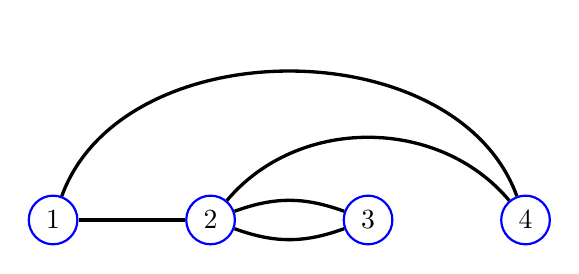
\begin{tikzpicture}[scale=2,very thick,block/.style ={circle, draw=blue, thick ,align=center, minimum height=0.3em}]
		\node[block] (n1) at (0,0) {1};
		\node[block] (n2) at (1,0) {2};
		\node[block] (n3) at (2,0) {3};
		\node[block] (n4) at (3,0) {4};
		\draw (n1)--(n2);
		\draw (n2) [out=20,in=160] to (n3);
		\draw (n2) [out=-20,in=-160] to (n3);
		\draw (n2) [out=50,in=130] to (n4);
		\draw (n4) [out=110,in=70] to (n1);
	\end{tikzpicture}
	\caption{Graph $G_w$ corresponding to the word $w=123241$.}
	\label{fig:Feynman_diag_ex}
\end{figure}

Let $N_{i_1i_2}^w$ be the number of distinct edges connecting $i_1$ to $i_2$ in $G_w$. In our running example we have $N_{12}^w=1$ and $N_{23}^w=2$.
Each edge may be a \emph{self} edge such as $(1,1)$, or it can be an edge \emph{connecting} distinct vertices such as $(2,3)$.

With this notation we have
\begin{equation}\label{WSCL_proof_1}
	\EE a_{i_1i_2}a_{i_2i_3}\cdots a_{i_{k-1}i_k}a_{i_ki_1}=
	\prod_{\substack{\textnormal{self $e$}\\e\in G_{i_1\ldots i_ki_1}}}\EE a_{11}^{N_e}
	\prod_{\substack{\textnormal{connecting $e$}\\ e\in G_{i_1\ldots i_ki_1}}}\EE a_{12}^{N_e},
\end{equation}
since all diagonal elements are iid, and all the elements above the diagonal are iid.
Here the product runs over all possible distinct edges in the graph of the word.

In order for the expectation
\eqref{WSCL_proof_1} to be nonzero, we must have the following properties:
\begin{itemize}
	\item
	Since $\EE a_{ij}=0$, each edge in $G_{i_1\ldots i_ki_1}$ must have 
	$N_e\ge2$..
	\item The graph $G_{i_1\ldots i_ki_1}$ has $k+1$ edges, and so it can have
	at most $1+k/2$ vertices.
\end{itemize}

Now let us look at the sum \eqref{WSCL_proof_0} as a whole. 
Call two graphs
\emph{equivalent}
if they differ only by relabeling the vertices.
Note that the 
expectations 
of the form
\eqref{WSCL_proof_1}
coming from equivalent graphs are the same. If a graph has $t$ vertices, then there are 
$N^{\downarrow t}:=N(N-1)\ldots(N-t+1)$ ways to relabel the vertices 
to get an equivalent graph. This implies that the sum
\eqref{WSCL_proof_0} can be rewritten as
\begin{align}\label{WSCL_proof_2}
	\EE\langle x^k, L_N\rangle=\sum_{t=0}^{1+\lfloor k/2\rfloor}\frac{N^{\downarrow t}}{N^{1+k/2}}
	\underbrace{\sum_{G_w\in\text{EqClass}_t}\,
	\prod_{\substack{\text{self } e\\e\in G_{w}}}\EE a_{11}^{N_e}
	\prod_{\substack{\text{connecting } e\\ e\in G_{w}}}\EE a_{12}^{N_e}}_{(*)},
\end{align}
where by $\text{EqClass}_t$ we have denoted the set of equivalence classes
of graphs $G_w$ corresponding to closed word, having $t$ vertices and $k+1$ edges, and 
also having $N_e\ge2$ for each edge.

Clearly, for fixed $t$ and $k$, the expression $(*)$ above does not depend on $N$
and is finite. Also, since $N^{\downarrow t}=O(N^{t})$, 
the sum \eqref{WSCL_proof_2} vanishes as $N\to\infty$
unless $t=1+k/2$. Because $t\le \lfloor k/2\rfloor$, this is possible only
for $k$ even. Therefore,
$\EE\langle x^k, L_N\rangle$ converges to zero if $k$ is odd.

Now consider the case when $k$ is even and $t=1+k/2$. Then the graph corresponding to each word
$i_1 \ldots i_ki_1$ has $k+1$ edges, $1+k/2$ vertices, 
and $N_e\ge2$ for each edge. Hence, gluing together pairs of edges connecting 
the same vertices, we see that the graph 
$G_{i_1 \ldots i_ki_1}$ must be a \emph{tree} (see \Cref{fig:Wigner_word}).\footnote{The words which correspond to
such trees 
contributing to \eqref{WSCL_proof_2}
are sometimes referred to as \emph{Wigner words}.}
In particular, there are no self edges and $N_e=2$ for each connecting edge. This implies that 
\begin{align*}
	\lim_{N\to\infty}\EE\langle x^k, L_N\rangle=\big|\text{EqClass}_{1+k/2}\big|.
\end{align*}

\begin{figure}[htbp]
	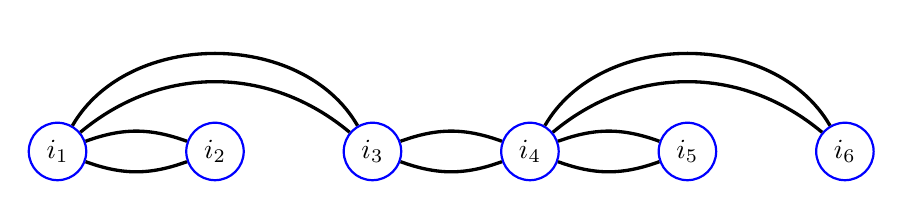
\begin{tikzpicture}[scale=2,very thick,block/.style ={circle, draw=blue, thick ,align=center, minimum height=0.3em}]
		\node[block] (n1) at (0,0) {$i_1$};
		\node[block] (n2) at (1,0) {$i_2$};
		\node[block] (n3) at (2,0) {$i_3$};
		\node[block] (n4) at (3,0) {$i_4$};
		\node[block] (n5) at (4,0) {$i_5$};
		\node[block] (n6) at (5,0) {$i_6$};
		\draw (n1) [out=20,in=160] to (n2);
		\draw (n1) [out=-20,in=-160] to (n2);
		\draw (n1) [out=40,in=140] to (n3);
		\draw (n1) [out=60,in=120] to (n3);
		\draw (n3) [out=20,in=160] to (n4);
		\draw (n3) [out=-20,in=-160] to (n4);
		\draw (n4) [out=20,in=160] to (n5);
		\draw (n4) [out=-20,in=-160] to (n5);
		\draw (n4) [out=40,in=140] to (n6);
		\draw (n4) [out=60,in=120] to (n6);
	\end{tikzpicture}
	\caption{A graph $G_w$ corresponding to a Wigner word 
	$w=i_{1}i_3i_4i_5i_4i_6i_4i_3i_1i_2i_1$
	which nontrivially contributes to the expansion \eqref{WSCL_proof_2}. 
	Here $k=10$.}
	\label{fig:Wigner_word}
\end{figure}	
\begin{figure}[htbp]
	\raisebox{50pt}{\scalebox{.8}{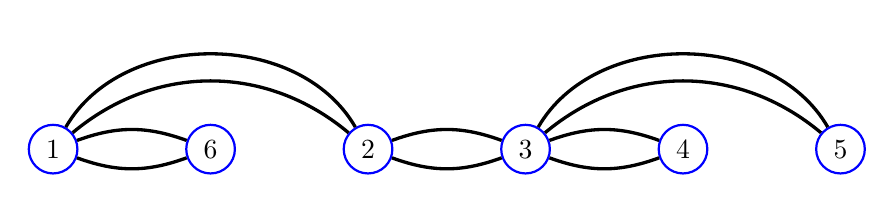
\begin{tikzpicture}[scale=2,very thick,block/.style ={circle, draw=blue, thick ,align=center, minimum height=0.3em}]
		\node[block] (n1) at (0,0) {$1$};
		\node[block] (n2) at (1,0) {$6$};
		\node[block] (n3) at (2,0) {$2$};
		\node[block] (n4) at (3,0) {$3$};
		\node[block] (n5) at (4,0) {$4$};
		\node[block] (n6) at (5,0) {$5$};
		\draw (n1) [out=20,in=160] to (n2);
		\draw (n1) [out=-20,in=-160] to (n2);
		\draw (n1) [out=40,in=140] to (n3);
		\draw (n1) [out=60,in=120] to (n3);
		\draw (n3) [out=20,in=160] to (n4);
		\draw (n3) [out=-20,in=-160] to (n4);
		\draw (n4) [out=20,in=160] to (n5);
		\draw (n4) [out=-20,in=-160] to (n5);
		\draw (n4) [out=40,in=140] to (n6);
		\draw (n4) [out=60,in=120] to (n6);
	\end{tikzpicture}}}
	\hspace{40pt}
	\scalebox{.8}{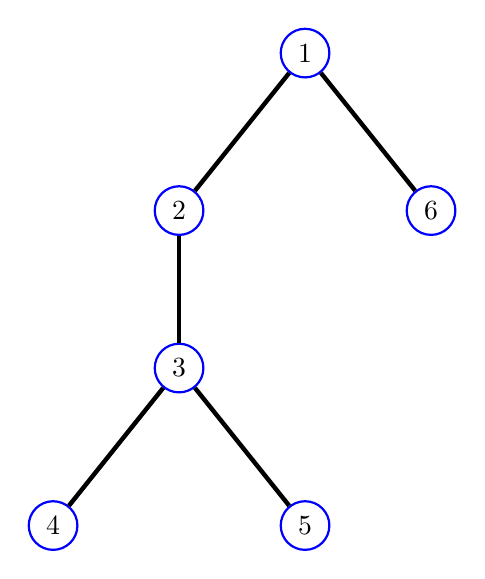
\begin{tikzpicture}[scale=2,very thick,block/.style ={circle, draw=blue, thick ,align=center, minimum height=0.3em}]
		\node[block] (n1) at (0,0) {$1$};
		\node[block] (n2) at (.8,-1) {$6$};
		\node[block] (n3) at (-.8,-1) {$2$};
		\node[block] (n4) at (-.8,-2) {$3$};
		\node[block] (n5) at (-1.6,-3) {$4$};
		\node[block] (n6) at (0,-3) {$5$};
		\draw[ultra thick] (n1)--(n3);
		\draw[ultra thick] (n1)--(n2);
		\draw[ultra thick] (n3)--(n4);
		\draw[ultra thick] (n4)--(n5);
		\draw[ultra thick] (n4)--(n6);
	\end{tikzpicture}}
	\caption{A representative graph 
	$G_w\in \text{EqClass}_{1+k/2}$ corresponding to the graph as in
	\Cref{fig:Wigner_word} (left), and its representation as a rooted ordered tree (right).}
	\label{fig:Wigner_word_representative}
\end{figure}

To count the number of trees $G_w\in\text{EqClass}_{1+k/2}$, 
let us choose representatives $w=v_1 \ldots v_{k+1}$,
such that for each $i=1,\ldots,k+1$, the set $\{1,2,\ldots,v_i\}$
is an interval in $\{1,2,\ldots,N\}$ beginning at $1$
(thus, $v_1=v_{k+1}=1$).
\begin{exercise}
	There is a unique way of choosing such representatives.
\end{exercise}
Let the vertex $1$ be the root $R$, and clearly the order coming from the word
defines an order on this rooted tree (see \Cref{fig:Wigner_word_representative}). This implies that 
$\big|\text{EqClass}_{1+k/2}\big|=\mathrm{Cat}_k$, and
finally proves the desired convergence \eqref{desired_convergence_of_averages_in_WSCL}.

% subsection convergence_of_expectations_ (end)

\lect{1/27/2016}

\subsection{An example of counting terms in the expansion of \cref{WSCL_proof_0}} % (fold)
\label{sub:an_example_WSCL_proof}

Before proceeding to finish the proof, let us consider one example 
how expansion \eqref{WSCL_proof_0} works 
for $k=6$.

\begin{exercise}
How go get $ \mathrm{Cat}_3 = 5 $ from $ \EE(\mathop{\mathrm{tr}}( A^6 ) )$ ?
\end{exercise}
\begin{proof}[Solution]
	We want to show how

	\begin{equation*}
	\EE( \, \text{tr}( A^6 ) \, ) = N^{ -1 - 3 } \sum_{ i_1 , \ldots, i_6 = 1 }^N \EE \left( a_{ i_1, i_2 } \cdot a_{ i_2, i_3 } \cdots a_{ i_5, i_6 } \cdot a_{ i_6, i_1 } \right) \xrightarrow[ N \to \infty ]{} 5.
	\end{equation*}

	We need to determine which terms are nonzero and how many such terms there are.  If there are 5 or 6 independent indices, we get a product of expected values of independent random variables with expected value zero, so these terms do not contribute.  If there are 3 or fewer independent indices, there are not enough terms to overcome the factor of $ N^{ -4 } $, so these terms do not contribute in the limit.  Thus we are interested in nonzero terms with 4 independent indices.
	One can check that there are 5 types of such terms:

	\begin{enumerate}

	\item
	\begin{equation*}
	\underbrace{ ( i_1, i_2 ) , ( i_2 , i_1 ) }, \quad \underbrace{ ( i_1, i_3 ) , ( i_3, i_1 ) }, \quad \underbrace{ ( i_1, i_4 ), ( i_4, i_1 ) }
	\end{equation*}

	\item
	\begin{equation*}
	\underbrace{ ( i_1, i_2 ) , \quad \underbrace{ ( i_2 , i_3 ) , ( i_3, i_2 ) } , \quad ( i_2, i_1 ) } , \quad \underbrace{ ( i_1, i_4 ), ( i_4, i_1 ) }
	\end{equation*}

	\item
	\begin{equation*}
	\underbrace{ ( i_1, i_2 ) , \quad \underbrace{ ( i_2 , i_3 ) , ( i_3, i_2 ) } , \quad \underbrace{ ( i_2, i_4 ) , ( i_4, i_2 ) }, \quad ( i_2, i_1 ) } 
	\end{equation*}

	\item
	\begin{equation*}
	\underbrace{ ( i_1, i_2 ) , \quad \underbrace{ ( i_2 , i_3 ) , \quad \underbrace{ ( i_3, i_4 ) , ( i_4, i_3 ) }, \quad ( i_3, i_2 ) } , \quad ( i_2, i_1 ) } 
	\end{equation*}

	\item
	\begin{equation*}
	\underbrace{ ( i_1, i_2 ) , ( i_2 , i_1 ) } , \quad \underbrace{ ( i_1, i_3 ) , \quad \underbrace{ ( i_3, i_4 ) , ( i_4, i_3 ) } , \quad ( i_3, i_1 ) }
	\end{equation*}

	\end{enumerate}

	These sequences bijectively correspond to noncrossing pair partitions of 6 elements.
	These partitions are in a clear bijection with Dyck paths of length 6
	(shown in \Cref{fig:Dyck3}), and are enumerated by the Catalan number $\mathrm{Cat}_3=5$.

	For each of these patterns, there are $ N ( N - 1 ) ( N - 2 ) ( N - 3 ) \sim N^4 $ terms in the sum, and each term is a product of the expected value of the squares of three independent off-diagonal random variables with expected value 0 and variance 1, like
	\begin{align*}
	\EE ( a_{ i_1, i_2 } \cdot a_{ i_2 , i_1 } \cdot a_{ i_1, i_3 } \cdot a_{ i_3, i_1 } \cdot a_{ i_1, i_4 } \cdot a_{ i_4, i_1 } ) &= \EE( a_{ i_1, i_2 }^2 ) \cdot \EE( a_{ i_1, i_3 }^2 ) \cdot \EE( a_{ i_1, i_4 }^2 ) = 1.
	\end{align*}
	So in the limit we get the Catalan number $ \mathrm{Cat}_3 = 5 $.
\end{proof}

% subsection an_example (end)

\subsection{Variances of $\langle x^k,L_N\rangle$} % (fold)
\label{sub:variances_langle_x_k_l_nrangleto0_}

Let us now show that the variances vanish in the limit:
\begin{equation}\label{Variance_to_zero_WSCL}
\EE ( \, \langle x^k , L_N \rangle^2 ) - \left( \, \EE ( \, \langle x^k , L_N \rangle \, ) \, \right)^2 \xrightarrow[ N \to \infty ]{} 0.
\end{equation}
Recall that
\begin{equation*}
\langle x^k , L_N \rangle = N^{ -1 - k/2 } \sum_{ \vec{i} = i_1 , \ldots, i_k = 1 }^n a_{ i_1, i_2 } \cdots a_{ i_k , i_1 }.
\end{equation*}
Now, writing $ a_{ \vec{i} } $ for $ a_{ i_1, i_2 } \cdots a_{ i_k , i_1 } $, we have
\begin{equation*}
\EE ( \, \langle x^k , L_N \rangle^2 ) - \left( \, \EE ( \, \langle x^k , L_N \rangle \, ) \, \right)^2 = N^{ -2 - k } \sum_{ \vec{i} , \vec{j} } \left(  \EE \left( a_{ \vec{i} } \cdot a_{ \vec{j} } \right) - \EE ( a_{ \vec{i} } ) \cdot \EE ( a_{ \vec{j} } ) \, \right).
\end{equation*}
If the graphs $ G_{ \vec{i} } $ and $ G_{ \vec{j} } $ 
(corresponding to the words $i_1 \ldots i_ki_1$ and $j_1 \ldots j_kj_1$,
respectively)
do not share common edges, 
then the corresponding random variables $ a_{ \vec{i} } $ and $ a_{ \vec{j} } $ 
are independent, and so $ \EE( a_{ \vec{ i } } \cdot a_{ \vec{j} } ) = \EE ( a_{ \vec{i} } ) \cdot \EE( a_{ \vec{j} } ) $.  
Thus we are only interested in the terms for which edges of the 
graphs $ G_{ \vec{i} } $ and $ G_{ \vec{j} } $ overlap.

\begin{example}\label{ex:GiGj_variance_in_WSCL}
	For instance, if $ \vec{i} = ( 1, 2, 3, 2 , 1 ) $ and $ \vec{j} = ( 1, 2, 1, 1, 1 ) $, then
	\begin{align*}
	\EE( a_{ \vec{i} } ) = \EE( a_{ i_1, i_2 } \cdot a_{ i_2, i_3 } \cdot a_{ i_3, i_2 } \cdot a_{ i_2, i_1 } ) &= \EE( a_{ 1, 2 }^2 )^2 = 1;
	\\\EE( a_{ \vec{j} } ) = \EE( a_{ i_1, i_2 } \cdot a_{ i_2, i_1 } \cdot a_{ i_1, i_1 } \cdot a_{ i_1, i_1 } ) &= \EE( a_{ 1, 2 }^2 ) \cdot \EE( a_{ 1,1 } ) = 2;
	\\\EE( a_{ i_1, i_2 } \cdot a_{ i_2, i_3 } \cdot a_{ i_3, i_2 } \cdot a_{ i_2, i_1 } \cdot a_{ i_1, i_2 } \cdot a_{ i_2, i_1 } \cdot a_{ i_1, i_1 } \cdot a_{ i_1, i_1 } ) &= \EE( a_{ i_1, i_2 }^4 ) \cdot \EE( a_{ i_2, i_3 }^2 ) \cdot \EE( a_{ i_1, i_1 }^2 ) = 2 \EE( a_{ 1, 2 }^4 ).
	\end{align*}
	The corresponding graphs are given in \Cref{fig:GiGj_variance_in_WSCL}.
\end{example}
\begin{figure}[htbp]
	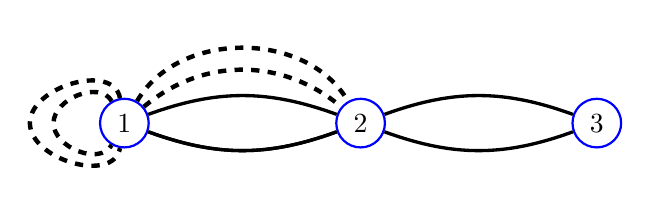
\begin{tikzpicture}[scale=3,very thick,block/.style ={circle, draw=blue, thick ,align=center, minimum height=0.3em}]
		\node[block] (n1) at (0,0) {$1$};
		\node[block] (n2) at (1,0) {$2$};
		\node[block] (n3) at (2,0) {$3$};
		\draw (n1) [out=20,in=160] to (n2);
		\draw (n1) [out=-20,in=-160] to (n2);
		\draw[dashed, ultra thick] (n1) [out=40,in=140] to (n2);
		\draw[dashed, ultra thick] (n1) [out=60,in=120] to (n2);
		\draw[dashed, ultra thick] (n1) [out=120,in=90] to (-.3,0) [out=-90,in=-120] to (n1);
		\draw[dashed, ultra thick] (n1) [out=100,in=90] to (-.4,0) [out=-90,in=-100] to (n1);
		\draw (n1) [out=-20,in=-160] to (n2);
		\draw (n2) [out=20,in=160] to (n3);
		\draw (n2) [out=-20,in=-160] to (n3);
	\end{tikzpicture}
	\caption{Graphs $ G_{ \vec{i} } $ (solid lines) and $ G_{ \vec{j} } $ (dashed lines) in \Cref{ex:GiGj_variance_in_WSCL}.}
	\label{fig:GiGj_variance_in_WSCL}
\end{figure}

We now argue similarly to the proof given in \Cref{sub:convergence_of_expectations_}
(for the convergence of the first moments). Namely, 
in order for $ \EE ( a_{ \vec{i} } \cdot a_{ \vec{j} } ) - \EE( a_{ \vec{i} } ) \EE( a_{ \vec{j} } ) $ to be nonzero 
we must have the following:
\begin{itemize}
	\item Since
	$ \EE( a_{ i j } ) = 0$,
	the graphs need to have $ N_e \ge 2 $;
	\item The graphs $ G_{ \vec{i} } $ and $ G_{ \vec{j} } $ need to share some edges.
\end{itemize}

If the combined graph has $ t $ vertices, there are $ N^{ \downarrow t } = N ( N - 1 ) \cdots ( N - t + 1 ) $ equivalent classes of graphs.  Thus, the variance takes the form
\begin{equation*}
\EE ( \, \langle x^k , L_N \rangle^2 ) - \left( \, \EE ( \, \langle x^k , L_N \rangle \, ) \, \right)^2 = N^{ -2 - k } \sum_{ t = 1 }^{ 2k } N^{ \downarrow t } \underbrace{ \left[ \sum_{ \substack{ \text{equiv. classes} \\ \text{ of graphs with} \\ \text{ $2k$ vertices } } } ( \text{finite products of finite moments} )\right] }_{ \text{ finite and independent of $N$ } }
\end{equation*}
Thus, we must have $ t \ge k + 2 $ in order to have a nonzero contribution as $ N \to \infty $.  
The associated graphs have $ N_e \ge 2 $ and are connected (since $ G_{ \vec{i} } $ and $ G_{ \vec{j} } $ are connected and overlap).
There are totally $ 2 k $ edges with multiplicities, thus  $\le k $ double edges.
We conclude that there are no such graphs, and so there are no nonzero contributions to the 
variance in the limit as $N\to\infty$. This 
completes the proof of \eqref{Variance_to_zero_WSCL}.

\begin{remark}
	Remark: by a similar argument, $ t = k + 1 $ also cannot contribute.
	Indeed, the combined graph of $ G_{ \vec{i} } $ and $ G_{ \vec{j} } $
	has $\le k$ double edges and $k+1$ vertices so it must be a tree
	(in the same sense of gluing edges as in \Cref{sub:convergence_of_expectations_} above).
	However, as $ G_{ \vec{i} } $ and $ G_{ \vec{j} } $ must also overlap (i.e., share common edges),
	there are no such trees.
	This implies a better estimate on the variance:
	\begin{equation*}
	\EE \left( \, \langle x^k , L_N \rangle^2 \, \right) - \EE \left( \, \langle x^k , L_N \rangle \, \right)^2 = O( N^{-2} ) ,
	\qquad
	N\to\infty.
	\end{equation*}
	This estimate can in fact be used to show almost-sure convergence to the semi-circular law.
\end{remark}

% subsection variances_langle_x_k_l_nrangleto0_ (end)

\subsection{Estimates and completing the proof} % (fold)
\label{sub:completing_the_proof_WSCL}

We want to show that for any continuous bounded function $f\in C_B(\mathbb R)$, the random
variables $\langle f, L_N\rangle$ converge in probability to 
$\langle f, \SC\rangle$ (this is further detailed in \eqref{WignerSemicircleLaw_langle}).
We have already shown that 
\begin{itemize}
	\item The moments converge: $\EE\langle x^{k}, L_N\rangle\to\langle x^k,\SC\rangle$.
	\item The variances
	vanish: 
	$\EE ( \langle x^k , L_N \rangle^2 ) - ( \EE \langle x^k , L_N \rangle )^2 \to0.$
\end{itemize}

We will also need the following a priori estimate that the empirical distributions
$L_N$ are concentrated around zero:
\begin{lemma}\label{lemma:WSCL_truncation}
	For all $ \varepsilon > 0 $ there exists $ B>0 $ so that
	\begin{equation*}
		\PP \left( \, \left \langle \, | x |^k \mathbf{1}_{ | x | > B } , L_N \right \rangle > \varepsilon \right) \xrightarrow[ N \to \infty ]{} 0.
	\end{equation*}
\end{lemma}
Here an everywhere below $\mathbf{1}_{A}$ denotes the indicator function of an event $A$, so the function $| x |^k \mathbf{1}_{ | x | > B }$ looks as in \Cref{fig:indicator_polynomial}.
\begin{proof}
	We will use the Markov (sometimes also called Chebyshev) inequality:
	\begin{equation*}
	\PP (  | X | > a ) < \frac{ \EE | X |  }{ a }\qquad \textnormal{for any $a>0$}.
	\end{equation*}
	Note that for $ | x | \ge B \ge 1 $,
	$x^{2k}=|x|^{k}|x|^{k}\ge B^{k}|x|^{k}$, hence
	$ | x |^k \le x^{ 2 k } / B^k $.  Now we have by the Markov inequality:
	\begin{align*}
	\PP \left( \, \left \langle | x |^k \mathbf{1}_{ | x | > B } , L_N \right \rangle > \varepsilon \right) &< \frac{ 1 }{ \varepsilon } \EE \left( \, \left \langle | x |^k \mathbf{1}_{ | x | > B } , L_N \right \rangle \, \right) \le \frac{ \EE \left( \, \langle x^{ 2k } , L_N \rangle \, \right) }{ \varepsilon B^k }.
	\end{align*}
	We know that
	\begin{equation*}
	\EE \left( \langle x^{2k} , L_N \rangle \, \right) \to \EE \left( \, \langle x^{ 2k } , \SC \rangle \, \right) = \mathrm{Cat}_k.
	\end{equation*}
	An easy (and in fact exact in the exponential order) 
	estimate for the Catalan numbers is
	\begin{align*}
	\mathrm{Cat}_k=\frac{1}{k+1}\binom{2k}{k} \le \sum_{ j = 0 }^{ 2k } \binom{2k}{j} = 2^{2k} = 4^k.
	\end{align*}
	Thus
	\begin{equation*}
	\limsup_{ N \to \infty } \PP \left( \, \left \langle | x |^k \mathbf{1}_{ | x | > B } , L_N \right \rangle > \varepsilon \right) \le \frac{ \mathrm{Cat}_k }{ \varepsilon B^k } \le \frac{ 4^k }{ \varepsilon B^k }.
	\end{equation*}
	As $ k $ grows, the left hand side grows. However, for $ B > 4 $ the right hand side decays to zero. Thus if we set
	\begin{equation*}
	\alpha_k = \limsup_{ N \to \infty } \PP \left( \, \left \langle | x |^k \mathbf{1}_{ | x | > B } , L_N \right \rangle > \varepsilon \right),
	\end{equation*}
	then
	$$
	0 \le \alpha_1 \le \alpha_2 \le \ldots \le \frac{ 4^k }{ \varepsilon B^k } \to 0.
	$$
	Thus, all the $ \alpha_k $ are zero. Since the probabilities are nonnegative, the desired result follows.
\end{proof}
\begin{figure}[htbp]
	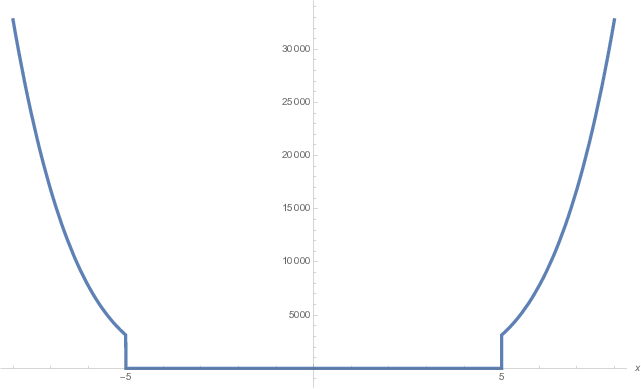
\includegraphics[width=.6\textwidth]{img/indicator_polynomial.png}
	\caption{The function $|x|^{5}\mathbf{1}_{|x|>5}$.}
	\label{fig:indicator_polynomial}
\end{figure}

Now, fix $B>4$ (say, $B=5$), and uniformly approximate the function 
$f\mathbf{1}_{|x|\le B}$ (a continuous function on a compact interval)
by a polynomial. That is, by the Weierstrass Approximation Theorem,
for every $\delta>0$ there is a polynomial
$Q_\delta(x)$ such that
\begin{align*}
	\sup_{|x|\le B}|f(x)-Q_{\delta}(x)|<\delta.
\end{align*}
Therefore, we can estimate
\begin{align*}
	\left|
	\langle f,L_N\rangle-
	\langle f,\SC\rangle
	\right|&\le
	\left|
	\langle f,L_N\rangle-
	\langle Q_{\delta},\SC\rangle
	\right|+
	\left|
	\langle Q_{\delta},\SC\rangle-
	\langle f,\SC\rangle
	\right|
	\\&\le
	\left|
	\langle f\mathbf{1}_{|x|\le B},L_N\rangle-
	\langle Q_{\delta},\SC\rangle
	\right|
	+
	\left|
	\langle f\mathbf{1}_{|x|> B},L_N\rangle
	\right|+
	\left|
	\langle Q_{\delta},\SC\rangle-
	\langle f,\SC\rangle
	\right|
	\\&\le
	\left|
	\langle Q_{\delta}\mathbf{1}_{|x|\le B},L_N\rangle-
	\langle Q_{\delta},\SC\rangle
	\right|\\&\hspace{20pt}+
	\left|
	\langle f\mathbf{1}_{|x|\le B},L_N\rangle-
	\langle Q_{\delta}\mathbf{1}_{|x|\le B},L_N\rangle
	\right|
	+
	\left|
	\langle f\mathbf{1}_{|x|> B},L_N\rangle
	\right|+
	\left|
	\langle Q_{\delta},\SC\rangle-
	\langle f,\SC\rangle
	\right|
	\\&\le
	\left|
	\langle Q_{\delta},L_N\rangle-
	\langle Q_{\delta},\SC\rangle
	\right|
	+
	\left|
	\langle Q_{\delta}\mathbf{1}_{|x|> B},L_N\rangle
	\right|\\&\hspace{20pt}+
	\left|
	\langle f\mathbf{1}_{|x|\le B},L_N\rangle-
	\langle Q_{\delta}\mathbf{1}_{|x|\le B},L_N\rangle
	\right|
	+
	\left|
	\langle f\mathbf{1}_{|x|> B},L_N\rangle
	\right|+
	\left|
	\langle Q_{\delta},\SC\rangle-
	\langle f,\SC\rangle
	\right|
	\\&\le
	\left|
	\langle Q_{\delta},L_N\rangle-
	\EE\langle Q_{\delta},L_N\rangle
	\right|
	+
	\left|
	\EE\langle Q_{\delta},L_N\rangle-
	\langle Q_{\delta},\SC\rangle
	\right|
	+
	\left|
	\langle Q_{\delta}\mathbf{1}_{|x|> B},L_N\rangle
	\right|\\&\hspace{20pt}+
	\left|
	\langle f\mathbf{1}_{|x|\le B},L_N\rangle-
	\langle Q_{\delta}\mathbf{1}_{|x|\le B},L_N\rangle
	\right|
	+
	\left|
	\langle f\mathbf{1}_{|x|> B},L_N\rangle
	\right|+
	\left|
	\langle Q_{\delta},\SC\rangle-
	\langle f,\SC\rangle
	\right|
	\\&\le
	\left|
	\langle Q_{\delta},L_N\rangle-
	\EE\langle Q_{\delta},L_N\rangle
	\right|
	+
	\left|
	\EE\langle Q_{\delta},L_N\rangle-
	\langle Q_{\delta},\SC\rangle
	\right|
	\\&\hspace{20pt}+
	\left|
	\langle Q_{\delta}\mathbf{1}_{|x|> B},L_N\rangle
	\right|+
	\left|
	\langle f\mathbf{1}_{|x|> B},L_N\rangle
	\right|+2 \delta.
\end{align*}
Therefore, we can estimate the probabilities as follows
(given that $\delta$ is sufficiently small):
\begin{align*}
	\PP\Big(\left|
	\langle f,L_N\rangle-
	\langle f,\SC\rangle
	\right|
	>\varepsilon\Big)&\le
	\PP\Big(
	\left|
	\langle Q_{\delta},L_N\rangle-
	\EE\langle Q_{\delta},L_N\rangle
	\right|>\varepsilon/5
	\Big)
	+
	\PP\Big(\left|
	\EE\langle Q_{\delta},L_N\rangle-
	\langle Q_{\delta},\SC\rangle
	\right|>\varepsilon/5\Big)
	\\&\hspace{40pt}+
	\PP\Big(\left|
	\langle Q_{\delta}\mathbf{1}_{|x|> B},L_N\rangle
	\right|>\varepsilon/5\Big)
	+
	\PP\Big(
	\left|
	\langle f\mathbf{1}_{|x|> B},L_N\rangle
	\right|>\varepsilon/5\Big).
\end{align*}
The first summand above convergences to zero by Chebyshev inequality:
\begin{align*}
	\PP\Big(
	\left|
	\langle Q_{\delta},L_N\rangle-
	\EE\langle Q_{\delta},L_N\rangle
	\right|>\varepsilon/5
	\Big)\le
	\frac{\EE\big(\langle Q_{\delta},L_N\rangle^{2}\big)
	-\big(\EE\langle Q_{\delta},L_N\rangle\big)^{2}}{(\varepsilon/5)^{2}},
\end{align*}
which goes to zero because variances go to zero
(\Cref{sub:variances_langle_x_k_l_nrangleto0_}).
The second summand convergences to zero because the moments
converge (\Cref{sub:convergence_of_expectations_}).
The last two summands converge to zero by
\Cref{lemma:WSCL_truncation} (note that $f$ is bounded and so 
can be bounded by a polynomial). 
This completes our first proof of the Wigner's semicircle law
(formulated above as \Cref{thm:SemicircleLaw}).

% subsection completing_the_proof (end)

\subsection{Related laws of large numbers for random matrix spectra} % (fold)
\label{sub:remarks_on_the_semicircle_law_for_real_wigner_matrices}

Let us mention two relatives of the Wigner semicircle law which can be proven by similar 
methods of moments and
trees counting.

\subsubsection{Complex Wigner matrices} % (fold)
\label{ssub:complex_wigner_matrices}
	
The first is the law of large numbers for complex (Hermitian) random Wigner
matrices $A= ( a_{ i j } )_{i,j=1}^{N}$, in which
\begin{itemize}
	\item $ \overline{ a_{ i j } } = a_{ j i } $, $i\le j$,
	are complex-valued independent random variables.
	\item The diagonal elements
	$ a_{ i i } $ are iid real valued with mean $0$ and variance $2$.
	\item $ a_{ i j } $ with $ i < j $ are iid complex random variables
	with expected value 0 and (complex) variance 1.
	On other words, $a_{ij}=x_{ij}+y_{ij}$, where $x_{ij}$ and $y_{ij}$ are independent
	real random variables with mean $0$ and variance $\frac12$. This implies that 
	$\EE a_{ij}^{2}=0$ and $\EE |a_{ij}|^{2}=1$.
	\item All moments $\EE|a_{ij}|^{k}$ are finite.
\end{itemize}
Defining $L_N$ in in the same way by \eqref{EmpiricalDistributionOfEigenvalues}
(note that the eigenvalues of $A$ are real because it is Hermitian),
we still have the semicircle law: 
$ L_N \rightarrow \SC $ weakly in probability. The proof of this result involves counting 
of graphs similarly to the real case described above, but in the case of Hermitian Wigner matrices
the graphs will be directed.

There also exist laws of large numbers
for complex eigenvalues of random matrices,
and typical is the \emph{circular law} stating
that the eigenvalues of a random matrix with iid 
entries are distributed uniformly inside a unit disc on the 
complex plane (cf. \Cref{rmk:complex_eigenvalues}).


% subsubsection complex_wigner_matrices (end)

\subsubsection{Marchenko--Pastur law} % (fold)
\label{ssub:marchenko_pastur_law}

The second relative is the Marchenko--Pastur law \cite{MarchenkoPastur}
for Wishart matrices (random sample covariance matrices). The Wishart ensemble is defined as follows.
Let $ Y $ be an $ N \times M $ matrix of iid real-valued random variables with mean 0 and variance 1. 
Then, by definition, $ W = Y Y^\text{T} $ is called a \emph{Wishart} $ N \times N $ random matrix.
It is a symmetric random matrix which is, moreover, positive definite.
Therefore, all its eigenvalues are real and nonnegative.
\begin{remark}
	If the entries of $ Y $ are Gaussian, then the entries of $ W $ are sums of squares of Gaussians, 
	so they have chi square distributions --- a type of distribution
	arising when studying sample covariance matrices of Gaussian random vectors.
\end{remark}

\begin{figure}[htbp]
	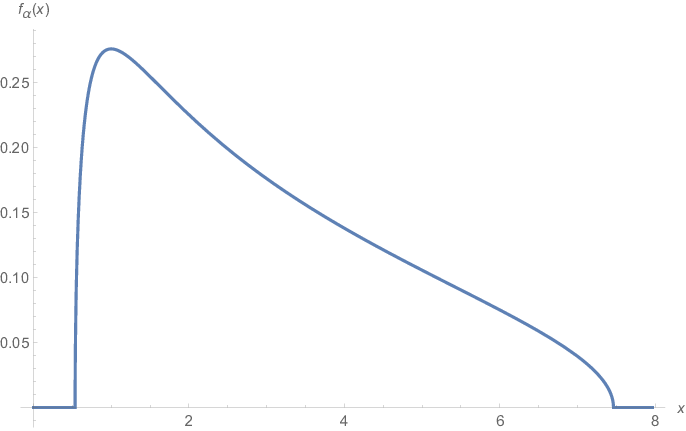
\includegraphics[width=.8\textwidth]{img/Marchenko-Pastur.png}
	\caption{The Marchenko--Pastur density $f_\alpha(x)$ for $\alpha=3$.}
	\label{fig:MP_law}
\end{figure}

Suppose $ M / N \to \alpha \in [ 1, \infty ) $. The Marchenko--Pastur law states that
\begin{equation*}
L_N = \frac{ 1 }{ N } \sum_{ i = 1 }^N \delta_{ \lambda_i / \sqrt{N} } \to S_\alpha 
\end{equation*}
weakly in probability. Here
$ S_\alpha $, $\alpha\in[1,\infty)$ are the Marchenko--Pastur distributions defined as follows.
Set
\begin{equation*}
b_\pm = ( 1 \pm \sqrt{\alpha} )^2.
\end{equation*}
Then the density function of $ S_\alpha $ is
\begin{equation*}
f_\alpha( x ) = \frac{ \sqrt{ ( x - b_- ) ( b_+ - x ) } }{ 2 \pi x }, \qquad b_- \le x \le b_+,
\end{equation*}
which looks as in \Cref{fig:MP_law}.

Note that if $ M \gg N $, then the random matrices $W$ are likely to be nondegenerate, so the distribution does not hit zero.
In fact, the distribution $ S_1 $ corresponding to $\alpha=1$
is the image of the semicircle law $ \SC $ under the squaring map $ x \mapsto x^2 $.

% subsubsection marchenko_pastur_law (end)

% subsection remarks_on_the_semicircle_law_for_real_wigner_matrices (end)

\subsection{Notes and references} % (fold)
\label{sub:notes_WSCL}

The combinatorial proof of the Wigner's semicircle law was essentially given by Wigner 
in \cite{wigner1955characteristic}. In our proof we closely follow Section 2.1 of
\cite{AndersonGuionnetZeitouniBook}.

% subsection notes (end)

% section wigner_s_semicircle_law (end)

\lect{2/1/2016}

\section{Elements of Free Probability} % (fold)
\label{sec:elements_of_free_probability}

\subsection{Motivating question} % (fold)
\label{sub:motivation}

We will discuss certain ideas from Free Probability
applied to spectra of random matrices. 
Our main goal is to motivate and describe the operation of free convolution
of two probability distributions with compact support. 
We will not discuss all the technical aspects and proofs, but will focus on 
certain concrete examples.

The motivating question we will be interested in is the following. Suppose
$A_N$ and $B_N$ are two ensembles of 
(real symmetric or Hermitian) $N\times N$ random matrices, and 
assume
\begin{equation*}
	L_N(A_N)\to\mu,\qquad L_N(B_N)\to\nu,
\end{equation*}
where $L_N$ is the empirical spectral distribution \eqref{EmpiricalDistributionOfEigenvalues}, and $\mu$ and $\nu$ are limiting probability measures on $\mathbb{R}$ with compact support.
The above convergence is the weak convergence in probability, as in 
\eqref{WignerSemicircleLaw} and \eqref{WignerSemicircleLaw_langle}.
The question is, how to understand the convergence of the sum:
\begin{equation*}
	L_N(A_N+B_N)\to\ ?
\end{equation*}
Of course, the answer will involve the dependence structure
of the ensembles $A_N$ and $B_N$, and here we will consider 
one choice of this dependence --- \emph{free independence},
which informally means that the eigenbases corresponding to the matrices
$A_N$ and $B_N$ are in generic position.
Then the empirical spectral distributions of $A_N+B_N$
converge to the \emph{free convolution}
$\mu\boxplus\nu$ of the measures $\mu$ and $\nu$.

\begin{example}
	Suppose $A_N$ and $B_N$ are independent and real Wigner. 
	Then by \Cref{thm:SemicircleLaw} we have
	$L_N(A_N)\to \SC$ and $L_N(B_N)\to \SC$. However, 
	$\displaystyle\frac{A_N+B_N}{\sqrt{2}}$ is also clearly real Wigner, and so
	\begin{equation*}
		L_N\left(\frac{A_N+B_N}{\sqrt{2}}\right) \to \SC.
	\end{equation*}
	We will see that this corresponds to the following
	rule for the free convolution:
	\begin{equation}\label{free_conv_SC}
		\frac{\SC\boxplus\SC}{\sqrt{2}}=\SC.
	\end{equation}

	In classical probability, if $X$ and $Y$ are iid random variables 
	such that for any constants $a,b$ we have 
	$aX+bY\stackrel{D}{=} cX+d$ for some other constants $c,d$, then $X$ is called
	\emph{stable}. An important such example is Gaussian random variables.
	Indeed, if  $X,Y$ are iid Gaussian random variables with mean $0$
	and variance $1$, then
	$X+Y=\sqrt{2}X$.  
	This suggests that the semicircle distribution should
	be the free analogue of the Gaussian distribution.
\end{example}

% subsection motivation (end)

\subsection{Classical moments and cumulants} % (fold)
\label{sub:classical_moments_and_cumulants}

Given a random variable $X$, the $n^{th}$ \emph{moment} of $X$ is
\begin{equation*}
	m_n(X)=\EE(X^n),\qquad n\geq 0.
\end{equation*}

\begin{definition}
The \emph{moment} (\emph{exponential}\footnote{The word
``exponential'' refers to the presence of the factorials in the series, which
resembles the Taylor series for the exponent $e^{z}$.}) \emph{generating function} for a random variable $X$ is given by 
\begin{align}\label{Moment_Gen}
\displaystyle M(z)=\EE (e^{z X})=\sum_{n=0}^\infty \frac{m_n(X)z^n}{n!}.
\end{align}
Let us define a new exponential generating function $C(z):=\log(M(z))$, and call its expansion coefficients $c_n(X)$, $n\ge1$,
the \emph{cumulants} of $X$:
\begin{align}\label{Cumulant_Gen}
\displaystyle C(z)=\sum_{n=1}^\infty \frac{c_n(X)z^n}{n!}=\log(M(z)).
\end{align}
\end{definition}

\begin{remark}
	When speaking of moments and cumulants, we will assume that the series \eqref{Moment_Gen} 
	converges for sufficiently small $z$, and that the moments define the distribution of $X$
	uniquely. A sufficient assumption which we will employ in this section unless otherwise
	noted is that all random variables (and probability distributions)
	have compact support.
\end{remark}

The cumulants (sometimes also called \emph{half/semi-invariants}) of $X$ form a sequence $(c_n)_{n\ge1}$, where $c_n$ is a homogeneous polynomial of moments $m_k$, $k\leq n$, with the leading term $m_n$:
\begin{equation}\label{skewness_kurtosis}
	\begin{split}
		c_1&=m_1=\EE X,\\
		c_2&=\VAR(X)=m_2-m_1^2,\\
		c_3&=\textnormal{skewness}=m_3-3m_2m_1+2m_1^3,\\
		c_4&=\textnormal{kurtosis}=m_4-4m_3m_1-3m_2^2+12m_2m_1^2-6m_1^4,\\
		&\vdots
	\end{split}
\end{equation}

\begin{example}[Cumulants of the Gaussian random variable]\label{ex:Cumulant_Seq_Ga}
	The moment generating function \eqref{Moment_Gen} of $\mathcal{N}(0,1)$, is 
	\begin{align*}
	    M(z)&= \int_{-\infty}^\infty e^{zx} \frac{e^{-x^2/2}}{\sqrt{2\pi}}\ dx\\
	    &=e^{z^2/2}\int_{-\infty}^\infty \frac{e^{-(x-z)^2/2}}{\sqrt{2\pi}}\ dx\\
	    &=e^{z^2/2}.
	\end{align*}
	Hence, the cumulant generating function \eqref{Cumulant_Gen} is 
	\begin{align*}
	    C(z)=z^2/2.
	\end{align*}
	This implies that the the cumulant sequence of $\mathcal{N}(0,1)$ is 
	\begin{align}\label{Cumulant_Seq_Ga}
	    (0, 1, 0, 0, ...).
	\end{align}
\end{example}

Now, if $X$ and $Y$ are independent random variables, then 
\begin{align*}
	c_2(X+Y)=\VAR(X+Y)=\VAR(X)+\VAR(Y)=c_2(X)+c_2(Y),
\end{align*}
so their second cumulants add up.
In fact, this holds for all higher cumulants, too:
\begin{proposition}
If $X$ and $Y$ are independent random variables, then for all $n\geq 1$, 
\begin{align}\label{lin_cumulants}
c_n(X+Y)=c_n(X)+c_n(Y).
\end{align}
\end{proposition}
\begin{proof}
	We have
	$M_X(z)=\EE e^{zX}$, so 
	$\EE(e^{zX+zY})=\EE e^{zX}\EE e^{zY}$
	by the usual product rule for expectations of independent
	random variables $e^{zX}$ and  $e^{zY}$, which implies
	$\log M_{X+Y}(z)=\log M_X(z)+\log M_Y(z)$, as desired.
\end{proof}

So, the cumuluants ``linearize'' addition of independent random variables. 
Note also that for $\alpha\in \mathbb{R}$, 
\begin{align}\label{lin_cumulants_2}
	c_n(\alpha X)=\alpha^nc_n(X).
\end{align}
To showcase the utility of the cumulants, we use them to prove the classical Central Limit Theorem (CLT):
\begin{theorem}[Central Limit Theorem]\label{thm:classic_clt}
	Let $X_1, X_2, ...$ be iid random variables with $\EE X_i=0$ (recall that we assume compact support). Then, 
	\begin{align*}
		S_N=\frac{X_1+...+X_N}{\sqrt{N}}\xrightarrow{\ D\ } \mathcal{N}(0,\VAR(X_1)).
	\end{align*}
\end{theorem}
\begin{proof}[Proof sketch]
	Note that, by \eqref{lin_cumulants} and \eqref{lin_cumulants_2}, for each $n$ and $N$, 
	\begin{align*}
	c_n(S_N)=N^{-n/2}Nc_n(X_1).
	\end{align*}
	In particular, we have:\footnote{The argument for $c_n(S_N)$ vanishing in the limit is similar to the one from 
	the proof of the Wigner's Semicircle Law, see 
	\eqref{WSCL_proof_2} in particular.} 
	\begin{align*}
	    n=1 :&\qquad  c_1(S_N) = \EE(X_1)=0,\\
	    n=2 :&\qquad  c_2(S_N) =c_2(X_1)=\VAR(X_1),\\
	     n\geq 3  :&\qquad c_n(S_N)\xrightarrow{N\to\infty} 0.
	\end{align*}
	So, the cumulant sequence of $\displaystyle \lim_{N\to\infty} S_N$ is 
	\begin{align}\label{Cumulant_seq_SN}
		(0, \VAR(X_1), 0, 0, ...).
	\end{align}
	By comparing \eqref{Cumulant_seq_SN} and \eqref{Cumulant_Seq_Ga}, we see that the cumulant sequences of $S_N$ and $\mathcal{N}(0,1)$ are the same up to a constant, which implies the CLT.
\end{proof}

% subsection classical_moments_and_cumulants (end)

\subsection{Moments and cumulants of Gaussian and semicircle distributions} % (fold)
\label{sub:moments_and_cumulants_of_gaussian_and_semicircle_distributions}

From \Cref{ex:Cumulant_Seq_Ga} we see that 
the moment generating function of $\mathcal{N}(0,1)$ is 
\begin{align*}
    M(z)=e^{z^2/2}=\sum_{n=0}^\infty \frac{z^{2n}}{2^nn!}=\sum_{k=0}^\infty \frac{m_k z^k}{k!}.
\end{align*}
Hence, $\mathcal{N}(0,1)$ has moments
\begin{align*}
    m_{2n+1} &=0,\\
    m_{2n}& = \frac{(2n)!}{2^nn!}=(2n-1)!!:=(2n-1)(2n-3)\cdots 3\cdot 1.
\end{align*}

Furthermore, we know from \eqref{m_2k_Catalan} that the semicircle distribution $\SC$ distribution has moments 
\begin{align*}
    m_{2n+1} &=0,\\
    m_{2n}& = \mathrm{Cat}_n=\frac{1}{n+1} {{2n}\choose{n}},
\end{align*}
where $\mathrm{Cat}_n$ is the $n$th Catalan number.
Now, we have the following correspondence:
\begin{equation*}
\begin{array}{llclcl}
\text{Classical:} &  \text{moments} & \longleftrightarrow &\  \text{cumulants} &\longleftrightarrow & \ \mathcal{N}(0,1) \ \text{has simplest cumulants}\\
\text{Random matrices:} & \text{moments} & \longleftrightarrow & ? &\longleftrightarrow &  \ \textnormal{``cumulants'' s.t. $\SC$ has simplest?}\\
\end{array}	
\end{equation*}

A natural question is how the cumulants of $\SC$ look like. Turns out they are not so nice. In fact, 
\begin{align*}
    \sum_{n=0}^\infty z^n \mathrm{Cat}_n=\frac{1-\sqrt{1-4z}}{2z},
\end{align*}
which is a good algebraic function. However, the moment exponential generating function
\eqref{Moment_Gen} 
for $\SC$ is more complicated:
\begin{align*}
    M(z)=\sum_{n=0}^\infty \frac{\mathrm{Cat}_nz^n}{n!}=e^{2z}(I_0(2z)-I_1(2z)),
\end{align*}
where the $I_k$'s are the modified Bessel functions of the first kind:
\begin{align*}
    I_\alpha(z)=\sum_{n=0}^\infty \frac{(z/2)^{\alpha+2n}}{n!\,\Gamma(n+1+\alpha)}.
\end{align*}
We thus will need a nicer analogue for cumulants.

% subsection moments_and_cumulants_of_gaussian_and_semicircle_distributions (end)

\subsection{Free cumulants} % (fold)
\label{sub:free_cumulants}

To explain the definition of free cumulants which replace the usual
cumulants in the context of random matrices in connection with the semicircle
distribution, let us first investigate the combinatorial relation between the 
moments and the classical cumulants in detail. That is, we 
want to generalize the formulas \eqref{skewness_kurtosis} to arbitrary $n$.
We will use the following combinatorial statement which can be found in 
\cite[Section 5.1]{Stanley1999}:
\begin{proposition}[Exponential formula]\label{prop:expon_thm}
	The moments can be expressed through cumulants as follows:
	\begin{equation}\label{moments_via_cumulants}
	     m_n=\sum_{\pi\in\mathcal{P}(n)} \prod_{B\in\pi} c_{|B|},
	\end{equation}
	where $\mathcal{P}(n)$ is the set of all partitions of the set 
	$\{1,...,n\}$, and $B\in \pi$ are the blocks of the partition $\pi$.
	See \Cref{fig:partition} for an example.
	\begin{figure}[htbp]
		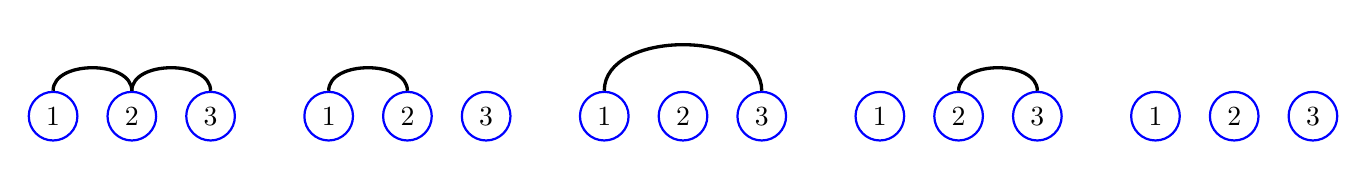
\begin{tikzpicture}
			[scale=1, very thick,block/.style ={circle, draw=blue, thick, align=center}]
			\begin{scope}[shift={(0,0)}]
				\node[block] (i1) at (0,0) {$1$};
				\node[block] (i2) at (1,0) {$2$};
				\node[block] (i3) at (2,0) {$3$};
				\draw (i1) to [out=90,in=90] (i2);
				\draw (i2) to [out=90,in=90] (i3);
			\end{scope}
			\begin{scope}[shift={(3.5,0)}]
				\node[block] (i1) at (0,0) {$1$};
				\node[block] (i2) at (1,0) {$2$};
				\node[block] (i3) at (2,0) {$3$};
				\draw (i1) to [out=90,in=90] (i2);
			\end{scope}
			\begin{scope}[shift={(7,0)}]
				\node[block] (i1) at (0,0) {$1$};
				\node[block] (i2) at (1,0) {$2$};
				\node[block] (i3) at (2,0) {$3$};
				\draw (i1) to [out=90,in=90] (i3);
			\end{scope}
			\begin{scope}[shift={(10.5,0)}]
				\node[block] (i1) at (0,0) {$1$};
				\node[block] (i2) at (1,0) {$2$};
				\node[block] (i3) at (2,0) {$3$};
				\draw (i2) to [out=90,in=90] (i3);
			\end{scope}
			\begin{scope}[shift={(14,0)}]
				\node[block] (i1) at (0,0) {$1$};
				\node[block] (i2) at (1,0) {$2$};
				\node[block] (i3) at (2,0) {$3$};
			\end{scope}
		\end{tikzpicture}
		\caption{All partitions of $\{1,2,3\}$, yielding the 
		expansion $m_3=c_3+3c_2c_1+c_1^{3}$.}
		\label{fig:partition}
	\end{figure}
\end{proposition}
This also implies that the cumulants can be recursively determined by the moments:
\begin{equation}\label{cumulants_via_moments}
	c_n=m_n-\sum_{\substack{\pi\in\mathcal{P}(n)\\\text{\# of blocks}\geq 2}} \prod_{B\in \pi} c_{|B|}.
\end{equation}
\begin{proof}
	We start with the identity of generating functions 
	\begin{equation}\label{M_exp_C}
		M(z)=\exp(C(z)),
	\end{equation}
	that is,
	\begin{equation*}
		\sum_{n=0}^{\infty}\frac{m_nz^{n}}{n!}=
		\sum_{k=0}^{\infty}\frac{(C(z))^{k}}{k!}.
	\end{equation*}
	Our aim is to use the definition of the exponential
	generating function $C(z)$ \eqref{Cumulant_Gen}
	to get the coefficient by $z^{n}$ from the right-hand side of the above identity
	of the generating functions. Write
	\begin{equation*}
		\frac{1}{k!}(C(z))^k=\frac1{k!}{\Big(\sum_{i=0}^\infty \frac{c_i z^i}{i!}\Big)^k}.
	\end{equation*}
	Take a partition $i_1,...,i_k$ of $n$, i.e. 
	$i_1+...+i_k=n$, 
	and take the $i_j$-th term from each bracket above.
	Then, we can write
	\begin{equation}
		\label{moment_multinomial_form}
		m_n=\sum_{\substack{k\\i_1,...,i_k}}\frac{c_{i_1}\cdots c_{i_k}n!}{k!i_1!\cdots i_k!}.
	\end{equation}
	Notice that $\displaystyle \frac{n!}{i_1!\cdots i_k!}$ is the multinomial coefficient,
	that is, the number of ways to put $n$ labeled objects into $k$
	labeled boxes, such that there are $i_j$ elements in the $j$th box. 
	Since in the set partition of $\{1,2,\ldots,n\}$
	the blocks are unlabeled, we have to divide this multinomial
	coefficient by $k!$ to get the number of the corresponding set partitions.
	With this perspective, we can rewrite the $n^{th}$ moment \eqref{moment_multinomial_form}
	as \eqref{moments_via_cumulants}, where $k$ is the number of the blocks of the partition
	$\pi$, and $i_1,\ldots,i_k$ are the sizes of these blocks.
\end{proof}

Applying \eqref{moments_via_cumulants} to the Gaussian distribution $\mathcal{N}(0,1)$, we have
\begin{equation}\label{gauss_via_cum}
	m_{2n}=(2n-1)!!=\sum_{\pi\in\mathcal{P}(2n)} \prod_{B\in\pi} c_{|B|}.
\end{equation}
However, since $c_n=0$ for $n\neq 2$ and $c_2=1$, the sum is only over pair partitions 
(i.e. partitions in which all blocks have size 2). Hence, 
\begin{align*}
 m_{2n}=(2n-1)!!=\# \Big\{\textnormal{pair partitions of $\{1,2,\ldots,2n\}$}\Big\}.
\end{align*}
See \Cref{fig:pair_partitions_NC_partitions}.
\begin{figure}[htbp]
		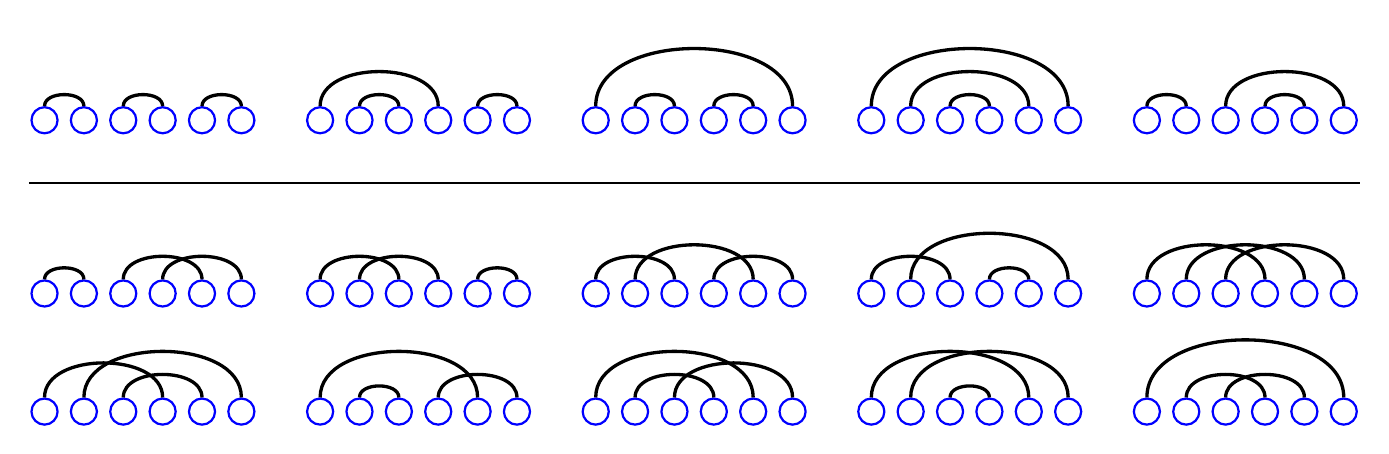
\begin{tikzpicture}
			[scale=1, very thick,block/.style ={circle, draw=blue, thick}]
			\draw[thick] (-.2,-.1)--(16.7,-.1);
			\begin{scope}[shift={(0,.7)}]
				\node[block] (i1) at (0,0) {};
				\node[block] (i2) at (.5,0) {};
				\node[block] (i3) at (1,0) {};
				\node[block] (i4) at (1.5,0) {};
				\node[block] (i5) at (2,0) {};
				\node[block] (i6) at (2.5,0) {};
				\draw (i1) to [out=90,in=90] (i2);
				\draw (i3) to [out=90,in=90] (i4);
				\draw (i5) to [out=90,in=90] (i6);
			\end{scope}
			\begin{scope}[shift={(3.5,.7)}]
				\node[block] (i1) at (0,0) {};
				\node[block] (i2) at (.5,0) {};
				\node[block] (i3) at (1,0) {};
				\node[block] (i4) at (1.5,0) {};
				\node[block] (i5) at (2,0) {};
				\node[block] (i6) at (2.5,0) {};
				\draw (i1) to [out=90,in=90] (i4);
				\draw (i2) to [out=90,in=90] (i3);
				\draw (i5) to [out=90,in=90] (i6);
			\end{scope}
			\begin{scope}[shift={(14,.7)}]
				\node[block] (i1) at (0,0) {};
				\node[block] (i2) at (.5,0) {};
				\node[block] (i3) at (1,0) {};
				\node[block] (i4) at (1.5,0) {};
				\node[block] (i5) at (2,0) {};
				\node[block] (i6) at (2.5,0) {};
				\draw (i1) to [out=90,in=90] (i2);
				\draw (i3) to [out=90,in=90] (i6);
				\draw (i4) to [out=90,in=90] (i5);
			\end{scope}
			\begin{scope}[shift={(7,.7)}]
				\node[block] (i1) at (0,0) {};
				\node[block] (i2) at (.5,0) {};
				\node[block] (i3) at (1,0) {};
				\node[block] (i4) at (1.5,0) {};
				\node[block] (i5) at (2,0) {};
				\node[block] (i6) at (2.5,0) {};
				\draw (i1) to [out=90,in=90] (i6);
				\draw (i2) to [out=90,in=90] (i3);
				\draw (i4) to [out=90,in=90] (i5);
			\end{scope}
			\begin{scope}[shift={(10.5,.7)}]
				\node[block] (i1) at (0,0) {};
				\node[block] (i2) at (.5,0) {};
				\node[block] (i3) at (1,0) {};
				\node[block] (i4) at (1.5,0) {};
				\node[block] (i5) at (2,0) {};
				\node[block] (i6) at (2.5,0) {};
				\draw (i1) to [out=90,in=90] (i6);
				\draw (i2) to [out=90,in=90] (i5);
				\draw (i4) to [out=90,in=90] (i3);
			\end{scope}

			\begin{scope}[shift={(0,-1.5)}]
				\node[block] (i1) at (0,0) {};
				\node[block] (i2) at (.5,0) {};
				\node[block] (i3) at (1,0) {};
				\node[block] (i4) at (1.5,0) {};
				\node[block] (i5) at (2,0) {};
				\node[block] (i6) at (2.5,0) {};
				\draw (i1) to [out=90,in=90] (i2);
				\draw (i3) to [out=90,in=90] (i5);
				\draw (i4) to [out=90,in=90] (i6);
			\end{scope}
			\begin{scope}[shift={(3.5,-1.5)}]
				\node[block] (i1) at (0,0) {};
				\node[block] (i2) at (.5,0) {};
				\node[block] (i3) at (1,0) {};
				\node[block] (i4) at (1.5,0) {};
				\node[block] (i5) at (2,0) {};
				\node[block] (i6) at (2.5,0) {};
				\draw (i1) to [out=90,in=90] (i3);
				\draw (i2) to [out=90,in=90] (i4);
				\draw (i5) to [out=90,in=90] (i6);
			\end{scope}
			\begin{scope}[shift={(7,-1.5)}]
				\node[block] (i1) at (0,0) {};
				\node[block] (i2) at (.5,0) {};
				\node[block] (i3) at (1,0) {};
				\node[block] (i4) at (1.5,0) {};
				\node[block] (i5) at (2,0) {};
				\node[block] (i6) at (2.5,0) {};
				\draw (i1) to [out=90,in=90] (i3);
				\draw (i2) to [out=90,in=90] (i5);
				\draw (i4) to [out=90,in=90] (i6);
			\end{scope}
			\begin{scope}[shift={(10.5,-1.5)}]
				\node[block] (i1) at (0,0) {};
				\node[block] (i2) at (.5,0) {};
				\node[block] (i3) at (1,0) {};
				\node[block] (i4) at (1.5,0) {};
				\node[block] (i5) at (2,0) {};
				\node[block] (i6) at (2.5,0) {};
				\draw (i1) to [out=90,in=90] (i3);
				\draw (i2) to [out=90,in=90] (i6);
				\draw (i4) to [out=90,in=90] (i5);
			\end{scope}
			\begin{scope}[shift={(14,-1.5)}]
				\node[block] (i1) at (0,0) {};
				\node[block] (i2) at (.5,0) {};
				\node[block] (i3) at (1,0) {};
				\node[block] (i4) at (1.5,0) {};
				\node[block] (i5) at (2,0) {};
				\node[block] (i6) at (2.5,0) {};
				\draw (i1) to [out=90,in=90] (i4);
				\draw (i2) to [out=90,in=90] (i5);
				\draw (i3) to [out=90,in=90] (i6);
			\end{scope}
			\begin{scope}[shift={(0,-3)}]
				\node[block] (i1) at (0,0) {};
				\node[block] (i2) at (.5,0) {};
				\node[block] (i3) at (1,0) {};
				\node[block] (i4) at (1.5,0) {};
				\node[block] (i5) at (2,0) {};
				\node[block] (i6) at (2.5,0) {};
				\draw (i1) to [out=90,in=90] (i4);
				\draw (i2) to [out=90,in=90] (i6);
				\draw (i3) to [out=90,in=90] (i5);
			\end{scope}
			\begin{scope}[shift={(3.5,-3)}]
				\node[block] (i1) at (0,0) {};
				\node[block] (i2) at (.5,0) {};
				\node[block] (i3) at (1,0) {};
				\node[block] (i4) at (1.5,0) {};
				\node[block] (i5) at (2,0) {};
				\node[block] (i6) at (2.5,0) {};
				\draw (i1) to [out=90,in=90] (i5);
				\draw (i2) to [out=90,in=90] (i3);
				\draw (i4) to [out=90,in=90] (i6);
			\end{scope}
			\begin{scope}[shift={(7,-3)}]
				\node[block] (i1) at (0,0) {};
				\node[block] (i2) at (.5,0) {};
				\node[block] (i3) at (1,0) {};
				\node[block] (i4) at (1.5,0) {};
				\node[block] (i5) at (2,0) {};
				\node[block] (i6) at (2.5,0) {};
				\draw (i1) to [out=90,in=90] (i5);
				\draw (i2) to [out=90,in=90] (i4);
				\draw (i3) to [out=90,in=90] (i6);
			\end{scope}
			\begin{scope}[shift={(10.5,-3)}]
				\node[block] (i1) at (0,0) {};
				\node[block] (i2) at (.5,0) {};
				\node[block] (i3) at (1,0) {};
				\node[block] (i4) at (1.5,0) {};
				\node[block] (i5) at (2,0) {};
				\node[block] (i6) at (2.5,0) {};
				\draw (i1) to [out=90,in=90] (i5);
				\draw (i2) to [out=90,in=90] (i6);
				\draw (i3) to [out=90,in=90] (i4);
			\end{scope}
			\begin{scope}[shift={(14,-3)}]
				\node[block] (i1) at (0,0) {};
				\node[block] (i2) at (.5,0) {};
				\node[block] (i3) at (1,0) {};
				\node[block] (i4) at (1.5,0) {};
				\node[block] (i5) at (2,0) {};
				\node[block] (i6) at (2.5,0) {};
				\draw (i1) to [out=90,in=90] (i6);
				\draw (i2) to [out=90,in=90] (i4);
				\draw (i3) to [out=90,in=90] (i5);
			\end{scope}
		\end{tikzpicture}
		\caption{All pair partitions of the set $\{1,2,3,4,5,6\}$.
		There are $5=\mathrm{Cat}_3$ noncrossing such partitions (the top $5$),
		and $15=5!!=5\cdot 3\cdot 1$ pair partitions in total.}
		\label{fig:pair_partitions_NC_partitions}
\end{figure}

Mimicking the classical Gaussian case, we would like to
find a class $\mathcal{P}'(2n)$ of partitions of the set $\{1,2,\ldots,2n\}$, such that the semicircle
moments have the form
\begin{equation}\label{cat_via_free_cum}
	\mathrm{Cat}_{n}=m_{2n}(\SC)=\sum_{\pi\in \mathcal{P}'(2n)}\prod_{B\in\pi} \kappa_{|B|},
\end{equation}
where $(\kappa_n)_{n\ge1}$ are the would-be free cumulants.
We want the semicircle distribution to have the simplest free cumulants, 
that, is, $\kappa_2=1$ and $\kappa_n=0$ for $n\ne2$.
Therefore, for the semicircle distribution
the sum in \eqref{cat_via_free_cum} must be over pair partitions from 
$\mathcal{P}'(n)$. 
\begin{quote}
	But we already know that the 
	Catalan number $\mathrm{Cat}_{n}$ counts the 
	number of \emph{noncrossing} pair partitions of $\{1,2,\ldots,2n\}$
	--- they are in a natural bijection with Dyck paths 
	of length $2n$ (cf. \Cref{sub:an_example_WSCL_proof}).
\end{quote}
The noncrossing pair partitions of $\{1,2,3,4,5,6\}$ are given in
\Cref{fig:pair_partitions_NC_partitions}, top.

This motivates the following general definition:
\begin{definition}[Free cumulants]
	Given a random variable $X$ with compact support and moments
	$m_n=\EE(X^{n})$, its \emph{free cumulants} are defined via the following expansion of moments
	\begin{equation}\label{free_cum_def}
		m_n=\sum_{\pi\in \mathcal{NC}(n)}\prod_{B\in\pi} \kappa_{|B|},
	\end{equation}
	where $\mathcal{NC}(n)$ is the set of noncrossing partitions of $\{1,2,\ldots,n\}$
	(cf. \Cref{fig:NC_part}).
\end{definition}
Clearly, rewriting \eqref{free_cum_def} similarly to \eqref{cumulants_via_moments} as
\begin{equation}\label{free_cum_via_mom}
	\kappa_n=m_n-\sum_{\substack{\pi\in\mathcal{NC}(n)\\\text{\# of blocks}\geq 2}} \prod_{B\in \pi} \kappa_{|B|},
\end{equation}
we see that the sequence of free cumulants $(\kappa_1,\kappa_2,\ldots)$
is uniquely determined by the sequence of moments.

	\begin{figure}[htbp]
		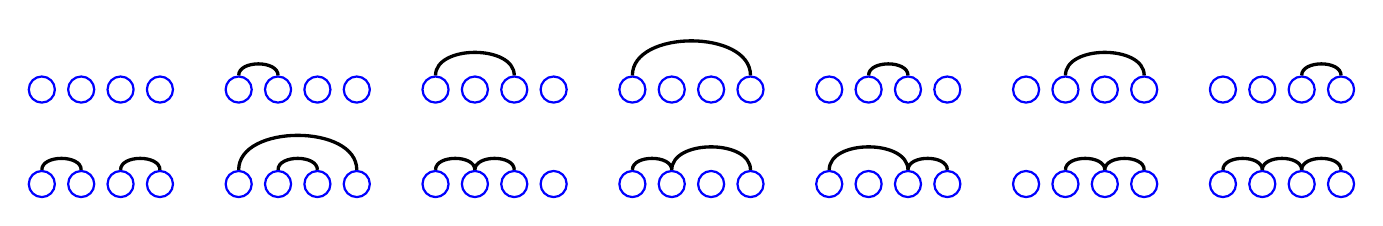
\begin{tikzpicture}
			[scale=1, very thick,block/.style ={circle, draw=blue, thick, align=center}]
			\begin{scope}[shift={(0,0)}]
				\node[block] (i1) at (0,0) {};
				\node[block] (i2) at (.5,0) {};
				\node[block] (i3) at (1,0) {};
				\node[block] (i4) at (1.5,0) {};
			\end{scope}
			\begin{scope}[shift={(2.5,0)}]
				\node[block] (i1) at (0,0) {};
				\node[block] (i2) at (.5,0) {};
				\node[block] (i3) at (1,0) {};
				\node[block] (i4) at (1.5,0) {};
				\draw (i1) to[out=90,in=90] (i2);
			\end{scope}
			\begin{scope}[shift={(5,0)}]
				\node[block] (i1) at (0,0) {};
				\node[block] (i2) at (.5,0) {};
				\node[block] (i3) at (1,0) {};
				\node[block] (i4) at (1.5,0) {};
				\draw (i1) to[out=90,in=90] (i3);
			\end{scope}
			\begin{scope}[shift={(7.5,0)}]
				\node[block] (i1) at (0,0) {};
				\node[block] (i2) at (.5,0) {};
				\node[block] (i3) at (1,0) {};
				\node[block] (i4) at (1.5,0) {};
				\draw (i1) to[out=90,in=90] (i4);
			\end{scope}
			\begin{scope}[shift={(10,0)}]
				\node[block] (i1) at (0,0) {};
				\node[block] (i2) at (.5,0) {};
				\node[block] (i3) at (1,0) {};
				\node[block] (i4) at (1.5,0) {};
				\draw (i2) to[out=90,in=90] (i3);
			\end{scope}
			\begin{scope}[shift={(12.5,0)}]
				\node[block] (i1) at (0,0) {};
				\node[block] (i2) at (.5,0) {};
				\node[block] (i3) at (1,0) {};
				\node[block] (i4) at (1.5,0) {};
				\draw (i2) to[out=90,in=90] (i4);
			\end{scope}
			\begin{scope}[shift={(15,0)}]
				\node[block] (i1) at (0,0) {};
				\node[block] (i2) at (.5,0) {};
				\node[block] (i3) at (1,0) {};
				\node[block] (i4) at (1.5,0) {};
				\draw (i3) to[out=90,in=90] (i4);
			\end{scope}
			\begin{scope}[shift={(0,-1.2)}]
				\node[block] (i1) at (0,0) {};
				\node[block] (i2) at (.5,0) {};
				\node[block] (i3) at (1,0) {};
				\node[block] (i4) at (1.5,0) {};
				\draw (i1) to[out=90,in=90] (i2);
				\draw (i3) to[out=90,in=90] (i4);
			\end{scope}
			\begin{scope}[shift={(2.5,-1.2)}]
				\node[block] (i1) at (0,0) {};
				\node[block] (i2) at (.5,0) {};
				\node[block] (i3) at (1,0) {};
				\node[block] (i4) at (1.5,0) {};
				\draw (i1) to[out=90,in=90] (i4);
				\draw (i2) to[out=90,in=90] (i3);
			\end{scope}
			\begin{scope}[shift={(5,-1.2)}]
				\node[block] (i1) at (0,0) {};
				\node[block] (i2) at (.5,0) {};
				\node[block] (i3) at (1,0) {};
				\node[block] (i4) at (1.5,0) {};
				\draw (i1) to[out=90,in=90] (i2) to[out=90,in=90] (i3);
			\end{scope}
			\begin{scope}[shift={(7.5,-1.2)}]
				\node[block] (i1) at (0,0) {};
				\node[block] (i2) at (.5,0) {};
				\node[block] (i3) at (1,0) {};
				\node[block] (i4) at (1.5,0) {};
				\draw (i1) to[out=90,in=90] (i2) to[out=90,in=90] (i4);
			\end{scope}
			\begin{scope}[shift={(10,-1.2)}]
				\node[block] (i1) at (0,0) {};
				\node[block] (i2) at (.5,0) {};
				\node[block] (i3) at (1,0) {};
				\node[block] (i4) at (1.5,0) {};
				\draw (i1) to[out=90,in=90] (i3) to[out=90,in=90] (i4);
			\end{scope}
			\begin{scope}[shift={(12.5,-1.2)}]
				\node[block] (i1) at (0,0) {};
				\node[block] (i2) at (.5,0) {};
				\node[block] (i3) at (1,0) {};
				\node[block] (i4) at (1.5,0) {};
				\draw (i2) to[out=90,in=90] (i3) to[out=90,in=90] (i4);
			\end{scope}
			\begin{scope}[shift={(15,-1.2)}]
				\node[block] (i1) at (0,0) {};
				\node[block] (i2) at (.5,0) {};
				\node[block] (i3) at (1,0) {};
				\node[block] (i4) at (1.5,0) {};
				\draw (i1) to[out=90,in=90] (i2);
				\draw (i2) to[out=90,in=90] (i3);
				\draw (i3) to[out=90,in=90] (i4);
			\end{scope}
		\end{tikzpicture}
		\caption{All noncrossing partitions of $\{1,2,3,4\}$, yielding the 
		expansion $m_4=\kappa_4+4\kappa_3\kappa_1+2\kappa_2^2+6\kappa_2\kappa_1^{2}+\kappa_1^{4}$.}
		\label{fig:NC_part}
	\end{figure}
Let us give a couple of remarks:
\begin{remark}
	For the ``simplest'' random variables --- Gaussian in the classical case and the 
	semicircle in the free case --- the sequence of cumulants or free cumulants, respectively,
	has the form
	\begin{equation*}
		(0,1,0,0,\ldots).
	\end{equation*}
	Therefore, the expansions \eqref{gauss_via_cum} and \eqref{cat_via_free_cum}
	involve only pair partitions. For general random variables 
	such expansions should involve all partitions with arbitrary part sizes.
\end{remark}
\begin{remark}
	Because all partitions are noncrossing for $n\leq 3$, we have
	 \begin{align*}
	     c_1& =\kappa_1,\\
	     c_2& =\kappa_2,\\
	     c_3& =\kappa_3.
	 \end{align*}
\end{remark}

% subsection free_cumulants (end)

\subsection{Example. Counting graphs} % (fold)
\label{sub:example_counting_graphs}

It is not essential that the quantities $m_n$ and $c_n$ in \Cref{prop:expon_thm}
are moments and cumulants of a certain random variable. 
Indeed, the exponential formula \eqref{moments_via_cumulants} holds
for coefficients of any exponential generating series related as 
\eqref{M_exp_C}.

The combinatorial meaning of the exponential formula \eqref{moments_via_cumulants}
is the following. If the quantities $m_n$ enumerate
certain kinds of objects on $n$ labeled vertices,
then the quantities $c_n$ related to $m_n$ via \eqref{moments_via_cumulants} 
or \eqref{cumulants_via_moments} count such objects which are \emph{connected}.

In particular, for counting undirected graphs on $n$ labeled vertices:
\begin{align*}
     m_n& =\# \ \text{of graphs}\ =2^{{n}\choose{2}},\\
     c_n& =\# \ \text{of connected graphs}.
\end{align*}
This property that the $c_n$'s count connected objects 
is clear from \eqref{moments_via_cumulants}: we count the total number
of objects by splitting each object into connected components
(this corresponds to picking a partition $\pi$),
and then counting the numbers of connected objects on vertices
inside these connected components.

Arguing in a similar way with the noncrossing cumulant formula \eqref{free_cum_def},
we see that if the moments $m_n=2^{\binom n2}$ count graphs, then the free cumulants
$\kappa_n$ count geometrically connected graphs on $n$ labeled vertices.
The geometrically connectedness condition naturally leads to splitting into noncrossing partitions.
See \Cref{fig:counting_graphs}.

\begin{figure}[htbp]
	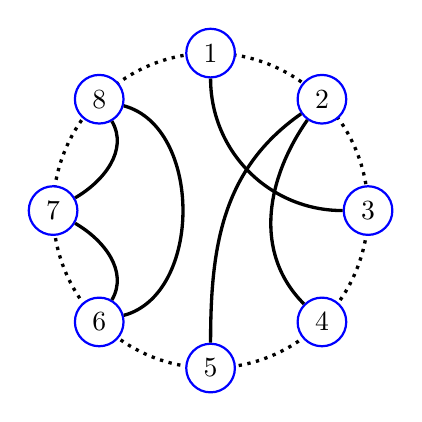
\begin{tikzpicture}[scale=1, very thick,block/.style ={circle, draw = blue, thick, fill=white, align = center}]
		\def\r{2};
		\def\rs{1.41421};
		\draw[dotted] (0,0) circle (\r);
		\node[block] (i1) at (0,\r) {$1$};
		\node[block] (i3) at (\r,0) {$3$};
		\node[block] (i7) at (-\r,0) {$7$};
		\node[block] (i5) at (0,-\r) {$5$};
		\node[block] (i2) at (\rs,\rs) {$2$};
		\node[block] (i4) at (\rs,-\rs) {$4$};
		\node[block] (i6) at (-\rs,-\rs) {$6$};
		\node[block] (i8) at (-\rs,\rs) {$8$};
		\draw (i1) to [out = -90,in = 180] (i3);
		\draw (i2) to [out = -145,in = 90] (i5);
		\draw (i2) to [out = -125,in = 135] (i4);
		\draw (i7) to [out = 30,in = -60] (i8);
		\draw (i7) to [out = -30,in = 60] (i6);
		\draw (i8) to [out = -15,in = 15] (i6);
	\end{tikzpicture}
	\caption{The geometric connectedness means that the graph on $n$ labeled vertices
	located on the circle is connected as a geometric figure if not as a graph. 
	The displayed graph has 3 connected and 2 geometrically connected components.}
	\label{fig:counting_graphs}
\end{figure}

% subsection example_counting_graphs (end)

\lect{2/3/2016}

\subsection{Free independence} % (fold)
\label{sub:free_independence}

Recall that in the classical case, for independent random variables $X$ and $Y$ and each $n\geq 1$,
\begin{align*}
    c_n(X+Y)=c_n(X)+c_n(Y).
\end{align*}
So, we would like to define free independence such that the same holds for free cumulants.
That is, if $X$ and $Y$ are free independent random variables, then for all $n\geq 1$,
\begin{align*}
    \kappa_n(X+Y)=\kappa_n(X)+\kappa_n(Y).
\end{align*}

To make a more precise definition of the free independence that we will work with, 
we need joint cumulants (classical and free).
That is, we want to speak not only about the variance and its higher analogues, 
but also about the covariance and its higher analogues (for two or more random variables).
This construction is rather straightforward: the joint moments are defined as
\begin{equation*}
	m_n(X_1,...,X_n)=\EE [X_1,...,X_n],
\end{equation*}
and the joint cumulants --- by the expansion
\begin{equation*}
	m_n(X_1,...,X_n)=\sum_{\pi\in\mathcal{P}(n)}\prod_{B\in\pi} c_{|B|}(X_i\colon i\in B).
\end{equation*}
To get the definition of the joint free cumulants, simply replace 
$\mathcal{P}(n)$ in the above formula by $\mathcal{NC}(n)$, and 
$c_{|B|}(X_i\colon i\in B)$
by
$\kappa_{|B|}(X_i\colon i\in B)$:
\begin{equation}\label{multilinear_mom_via_free_cum}
	m_n(X_1,...,X_n)=\sum_{\pi\in\mathcal{NC}(n)}\prod_{B\in\pi} \kappa_{|B|}(X_i\colon i\in B).
\end{equation}
Note that from \eqref{multilinear_mom_via_free_cum}
(more precisely, rewriting \eqref{multilinear_mom_via_free_cum}
in a recursive form like \eqref{free_cum_via_mom})
we see that $\kappa_n$ is a symmetric multilinear function of its arguments.

\begin{definition}[Free independence of classical random variables]\label{def:free_indep_classical}
	Two random variables $X$ and $Y$ 
	with $\EE X=\EE Y=0$
	are said to be 
	\emph{free independent} if all their joint mixed free cumulants vanish for all $n\ge2$:
	\begin{equation*}
		\kappa_n(X,Y,Y,\ldots,Y,Y)=
		\kappa_n(X,X,Y,\ldots,Y,Y)=\ldots=
		\kappa_n(X,X,X,\ldots,X,Y)=0.
	\end{equation*}
\end{definition}
    
\begin{exercise}
	Two random variables $X$ and $Y$ 
	with $\EE X=\EE Y=0$
	are classically independent
	if and only if all their joint mixed classical cumulants are zero:
	$c_n(X,X,...X,Y,...,Y)=0$.
\end{exercise}

\begin{example}
	Note that this will not be the same as regular independence. Indeed, 
	if you have two free independent $\SC$ random variables $X$ and $Y$, then
	\begin{align*}
	    X+Y\stackrel{D}{=} \sqrt 2\cdot \SC.
	\end{align*}
	For classically independent 
	$X$ and $Y$, their sum $X+Y$ clearly
	does not have the distribution $\sqrt 2\cdot \SC$
	(in particular,
	$\SC$ is not a stable distribution).
\end{example}

It turns out that free independence of classical random variables is problematic. 
To see this, consider free independent classical random variables $X$ and $Y$. Then, 
\begin{align*}
    m_4(X,X,Y,Y) = m_4(X,Y,X,Y),
\end{align*}
 where 
\begin{align*}
 m_4(X,X,Y,Y)=\kappa_2(X,X)\kappa_2(Y,Y)+\kappa_2(X,X)+\kappa_1(Y)^2 +\kappa_2(Y,Y)\kappa_1(X)^2+\kappa_1(X)^2\kappa_1(Y)^2,
\end{align*}
and
\begin{align*}
 m_4(X,Y,X,Y)=\kappa_2(X,X)\kappa_1(Y)^2+\kappa_1(X)^2\kappa_2(Y,Y)+\kappa_1(X)^2\kappa_2(Y)^2.
\end{align*}
Hence $\kappa_2(X,X)\kappa_2(Y,Y)=0$, which means that, for classical random variables, free independence requires one of the random variables to be constant. 

The solution is to introduce noncommutativity, whence
\begin{align*}
    m_4(X,X,Y,Y) \neq m_4(X,Y,X,Y),
\end{align*}
and, in fact, $XXYY\ne XYXY$.
This is the motivation for the definitions in the following subsection.

% subsection free_independence (end)

\subsection{Noncommutative spaces of random variables} % (fold)
\label{sub:free_random_variables}

The idea of free random variables was invented by Voiculescu in the beginning of the 
1980s, cf. \cite{Voiculescu_Free_book}. 
The space $L^\infty(\Omega, \mathcal{F},\PP)$ of bounded random variables 
is a commutative von Neumann algebra. 
Hence, noncommutative random variables would live in a noncommutative von Neumann algebra. 

To define a von Neumann algebra, first, let $H$ be a Hilbert space (complete inner product space over $\mathbb{C}$) and $\mathcal{B}(H)$ be the space of all bounded linear operators on $H$ (bounded with respect to the norm induced by the inner product $(\cdot|\cdot)$ on $H$). The space $\mathcal{B}(H)$ has a natural involution given by 
\begin{align*}
    (Tx|y)=(x|T^*y)
\end{align*}
for any $T\in \mathcal{B}(H)$ and $x,y\in H$. Elements of $\mathcal{B}(H)$
of the form $T^{*}T$ are called \emph{nonnegative}.

In addition to the topology on $\mathcal{B}(H)$ induced by the norm, there is a \emph{weak operator topology}. We say that for $T_n, T\in \mathcal{B}(H)$, $T_n\to T$ as $n\to\infty$
in the weak operator topology if for any $x,y\in H$,
\begin{align*}
    (T_nx|y)\to (Tx|y),\qquad n\to\infty.
\end{align*}
\begin{definition}
	A \emph{von Neumann algebra} $\mathcal{A}$
	is a unital (i.e., $1\in\mathcal{A}$) $*$-closed subalgebra 
	of $\mathcal{B}(H)$, which is closed with respect to the weak operator topology.
\end{definition}
We would
like to replace $L^\infty(\Omega, \mathcal{F}, \PP)$ with a von Neumann algebra $\mathcal{A}$.
To complete the picture, we would need an analogue of the expectation
which in the commutative case comes from the probability distribution.
In lieu of the classical expectation, we have a notion of tracial state on our von Neumann algebra. 

We will not consider the most general definition of a tracial state on a
von Neumann algebra, but will deal with functionals
$\tau\colon \mathcal{A}\to\mathbb{C}$ satisfying
\begin{enumerate}
    \item $\tau(1)=1$;
    \item $\tau(ab)=\tau(ba)$ for all $a,b\in\mathcal{A}_+$ (here $\mathcal{A}_+$
    is the subset of nonnegative elements in $\mathcal{A}$);
    \item $\tau(a^*a)\ge0$ for all $a\in\mathcal{A}$.
\end{enumerate}
The tracial state is \emph{faithful} if $\tau(a^*a)=0$ implies $a=0$.

So, we have the following correspondences:
\begin{equation*}
\begin{array}{c|c}
    \text{Classical} & \text{Noncommutative} \\ \hline
     L^\infty(\Omega, \mathcal{F}, P) & \text{a von Neumann algebra} \ \mathcal{A}\\
     \EE[\cdot] & \tau[\cdot]\\
     m_n(X) & m_n(a)=\tau(a^n),\ a\in \mathcal{A}_+
\end{array}	
\end{equation*}

Now, we define free independence for noncommutative random variables. 
\begin{definition}
Elements $a$ and $b$ in a von Neumann algebra $\mathcal{A}$ are \emph{free independent} if for any polynomials $f_1,g_1,..., f_k, g_k$ such that $\tau(f_i(a))=\tau(g_j(b))=0$, we have 
\begin{align*}
    \tau(f_1(a)g_1(b)f_2(a)g_2(b)\cdots g_k(b))=0.
\end{align*}
Note that this is essentially mimicking \Cref{def:free_indep_classical} 
stating that joint mixed cumulants are zero. 
\end{definition}
Compare this to the classical independence:
\begin{definition}
Elements $a$ and $b$ in a von Neumann algebra $\mathcal{A}$ are \emph{classically independent} if $ab=ba$ and for any polynomials $f$ and $g$ such that $\tau(f(a))=\tau(g(b))=0$, we have 
\begin{align*}
    \tau(f(a)g(b))=0.
\end{align*}
\end{definition}
If the moments $m_n(a)$ of an element $a\in\mathcal{A}$
can be identified with moments of a compactly supported probability distribution on $\mathbb{R}$,
we will denote this distribution by $\mu_a$.
That is, talking about a single random variable yields the same results
in commutative or noncommutative setting.
\begin{definition}[Free convolution]\label{def:free_convolution}
	If $a,b\in\mathcal{A}$ are free independent and correspond to compactly
	supported probability distributions $\mu_a$ and $\mu_b$ on $\mathbb{R}$, respectively,
	then their sum $a+b$ corresponds to a new 
	compactly
	supported probability distribution $\mu_{a+b}$ on $\mathbb{R}$. 
	This distribution $\mu_{a+b}$ is called the \emph{free convolution}
	of the distributions $\mu_a$ and $\mu_b$, and is denoted by 
	\begin{align*}
		\mu_{a+b}=\mu_a\boxplus\mu_b.
	\end{align*}
	As we will see below in \Cref{prop:asymptotically_free}
	and \Cref{sub:free_convolution_and_voiculescu_s_algorithm}, working with free convolution 
	does not require von Neumann algebras.
\end{definition}


To apply free probability to random matrices, we will need the following definition:
\begin{definition}
For a sequence $(\mathcal{A}_N,\tau_N)$ of von Neumann algebras with tracial states, and sequences $(a_N)$ and $(b_N)$ with $a_N, b_N\in \mathcal{A}_N$ 
for each $N$, we say that $(a_N)$ and $(b_N)$ are \emph{asymptotically free} if 
for all polynomials $f_1,g_1,..., f_k, g_k$ such that $\tau(f_i(a_N))\to 0$ and $\tau(g_j(b_N))\to0$, we have 
\begin{align*}
    \tau(f_1(a_N)g_1(b_N)f_2(a_N)g_2(b_N)\cdots g_k(b_N))\to 0.
\end{align*}
\end{definition}

An example of a sequence $(\mathcal{A}_N,\tau_N)$ of von Neumann algebras is 
given by random matrices. Take
$\mathcal{A}_N$ to be the von Neumann algebra of Hermitian
random matrices with almost surely bounded entries.\footnote{One can also take real symmetric random
matrices as we did in \Cref{sec:wigner_s_semicircle_law}. However,
from now on we will mostly work with Hermitian complex matrices, so we are 
switching to this setting.}
Equip each $\mathcal{A}_N$ with a tracial state
\begin{equation*}
	\tau_N(A):=\frac{1}{N} \EE \text{tr}(A),\qquad A\in\mathcal{A}_N,
\end{equation*}
coming from the usual matrix trace. 
Recall that quantities like $\tau_N(A)$ played a major role in the proof of the
Wigner's semicircle law in \Cref{sec:wigner_s_semicircle_law}.

\begin{proposition}\label{prop:asymptotically_free}
	Consider sequences $(A_N), (B_N)$ of $N\times N$ Hermitian random matrices from $\mathcal{A}_N$ with 
	\begin{align*}
		L_N(A_N)\to \mu ,\qquad L_N(B_N)\to \nu,
	\end{align*}
	as discussed in \Cref{sub:motivation}. Assume that $\mu$ and $\nu$ are compactly supported.
	For each $N$, let $U_N$ be the random Haar-distributed unitary matrix 
	that is independent of $A_N$ and $B_N$. 

	Then the random matrices $A_N$ and $U_NB_NU^*_N$ from $\mathcal{A}_N$ 
	are asymptotically free.  
\end{proposition}
\begin{proof}
	We will not prove this statement as it requires a graph enumeration somewhat similar to the proof 
	of the semicircle law. See, e.g., \cite[\S 3.6]{Novak2012FreeLectures} for an outline of the proof
	and more references.
\end{proof}

This proposition shows that the abstract definition of the free convolution (\Cref{def:free_convolution})
can be realized more concretely using summation of random matrices, one of which is randomly rotated, 
so that the eigenbases of $A_N$ and $U_NB_NU^*_N$ are in ``completely generic'' position.

% subsection free_random_variables (end)

\subsection{Semicircle law again} % (fold)
\label{sub:semicircle_law_again}

Using \Cref{prop:asymptotically_free}, we can give another proof of the 
Wigner's semicircle law, now for the Gaussian Unitary Ensemble (GUE).
First, note that a free analogue of the Central Limit theorem
states that if $X_1,X_2,\ldots$ is a family of free independent 
identically distributed elements of $(\mathcal{A},\tau)$
with mean $0$ and variance $1$,\footnote{That is,
$\tau(X_1)=0$ and $\tau(X_1^{2})=1$.} then
\begin{equation*}
	\frac{X_1+...+X_N}{\sqrt{N}}\to \SC,\qquad N\to\infty,
\end{equation*}
in the sense that for any $n\ge0$ we have
\begin{equation}\label{free_clt_moment_convergence}
	\tau\bigg[\Big(\frac{X_1+...+X_N}{\sqrt{N}}\Big)^{n}\bigg]\to m_n(\SC)=
	\begin{cases}
		0,&\textnormal{$n$ odd};\\
		\mathrm{Cat}_{n/2},
		&\textnormal{$n$ even}.
	\end{cases}
\end{equation}
This is proven using free cumulants exactly in the same way as in
the proof of the classical Central Limit Theorem using the classical
cumulants (\Cref{thm:classic_clt}).
	
Let us now sketch a proof of the semicircle law for the Gaussian Hermitian matrices.
Let $G_N$ be an $N\times N$ GUE random matrix (i.e., an Hermitian random
matrix with iid standard real Gaussians on the diagonal, 
and iid standard complex Gaussians --- with independent
real and imaginary parts having Gaussian distribution with variance $\frac 12$
--- above the diagonal). We would like to show that
$L_N(G_N)\to\SC$ weakly in probability. We have seen in \Cref{sec:wigner_s_semicircle_law} that
for this it is enough to show the convergence of the moments as in \eqref{free_clt_moment_convergence}.
Let $G_N^{(1)},...,G_N^{(N)}$ be independent copies of $G_N$.
By the unitary invariance of the GUE (see \Cref{sub:definition_and_basic_properties} below), for 
for $U_N^{(k)}, 1\leq k\leq N$ Haar-distributed unitary matrices independent of everything else, we have 
$U_N^{(k)}G_N^{(k)}(U_N^{(k)})^*\stackrel{D}{=} G_N$.
Furthermore, we clearly have by the Gaussian nature of the elements of the matrix:
\begin{align*}
    G_N\stackrel{D}{=}\frac{U_N^{(1)}G_N^{(1)}(U^{(1)}_N)^*+...+U_N^{(N)}G_N^{(N)}(U_N^{(N)})^*}{\sqrt{N}}.
\end{align*}
Finally, by \Cref{prop:asymptotically_free},
the summands above are asymptotically free. Thus, by the free CLT,
$L_N(G_N)$ converges to the semicircle distribution $\SC$. 

% subsection semicircle_law_again (end)

\subsection{Free convolution and Voiculescu's algorithm} % (fold)
\label{sub:free_convolution_and_voiculescu_s_algorithm}

Let us now describe the operation of the free convolution $(\mu,\nu)\mapsto \mu\boxplus \nu$
of \Cref{def:free_convolution}
(where $\mu$ and $\nu$ are probability distributions on $\mathbb{R}$ with compact
support) in more concrete terms.

We would like to describe an algorithm for computing $\mu\boxplus \nu$ given $\mu$ and $\nu$.
Recall that under free convolution we have $\kappa_n(\mu\boxplus\nu)=\kappa_n(\mu)+\kappa_n(\nu)$ for each $n\ge1$. 
We will use the following fact relating (ordinary, not exponential) moment generating function of a measure
and its free cumulant generating function:
\begin{equation}\label{L_K_definitions}
	L(z)=1+\sum_{n=1}^\infty m_nz^n,\qquad
	K(z)=1+\sum_{n=1}^\infty \kappa_nz^n,
\end{equation}
\begin{proposition}\label{prop:free_expon_thm}
	Thus defined generating series are related as follows:
	\begin{equation}\label{L_K_relations}
		L(z)=K\big(zL(z)\big).
	\end{equation}
\end{proposition}
\begin{proof}
	This is the free analogue of the exponential formula (\Cref{prop:expon_thm}),
	which can be proven by combinatorial manipulations with generating series.
	We will not give its proof here.
\end{proof}
\begin{remark}\label{rmk:L_K_inversion_exists}
	Relation \eqref{L_K_relations} between infinite power series can be used to compute coefficients
	of $L(z)$ if the coefficients of $K(z)$ are known, and vice versa. This is done in a purely formal way,
	by recursively looking at coefficients by powers of $z$ in both sides. Thus, \eqref{L_K_relations} 
	shows that moments and free cumulants uniquely determine each other.
	Of course, this uniqueness already follows from the combinatorial relations 
	\eqref{free_cum_def} and \eqref{free_cum_via_mom}. 
\end{remark}

Now, take the \emph{Cauchy transform} (sometimes also called the \emph{Stieltjes transform}) of each measure:
\begin{align*}
    G_\mu(z)&=\int_\mathbb{R} \frac{d\mu(x)}{z-x}\\
    &=\int_\mathbb{R} \frac{z^{-1} d\mu(x)}{1-x/z}\\
    &=\int_\mathbb{R}\sum_{n=0}^\infty z^{-1}\frac{x^n}{z^n} d\mu(x)\\
    &=\sum_{n=0}^\infty \int_\mathbb{R}z^{-1}\frac{x^n}{z^n} d\mu(x)\\
    &=\sum_{n=0}^\infty \frac{m_n(\mu)}{z^{n+1}}
\end{align*}
for large enough $|z|$, and similarly for $G_\nu(z)$
(recall that the measures have finite support).
Using \eqref{L_K_definitions} and \Cref{prop:free_expon_thm},
define
\begin{align*}
    V_{\mu}(z):=\frac{1}{z}K_{\mu}(z),
\end{align*}
and similarly for $\nu$. 
\Cref{prop:free_expon_thm} readily implies that
the functions $G_\mu$ and $V_\mu$ are mutual inverses:
\begin{equation}\label{V_G_relation}
	V_\mu\big(G_\mu(z)\big)=G_\mu\big(V_\mu(z)\big)=z.
\end{equation}

\begin{example}[Semicircle distribution]\label{G_SC}
We can compute $G_{\SC}$ using the Cauchy Transform:
\begin{align*}
G_{\SC}(z)&=\int_{-2}^2 \frac{\frac{1}{2\pi}\sqrt{1-4x^2}}{z-x}dx\\
&=\sum_{n=0}^\infty \frac{\mathrm{Cat}_n}{z^{2n+1}}\\
&=\frac{1}{z}\left(\frac{1-\sqrt{1-4/z^2}}{2}\right)\\
&=\frac{1}{2}z-\frac{1}{2}\sqrt{z^2-4}.
\end{align*}
We have computed this using the explicit formula for the Catalan numbers \eqref{Catalan_def}. This expansion can be 
verified by simply Taylor expanding $\frac{1}{2}z-\frac{1}{2}\sqrt{z^2-4}$ at $z=\infty$.

On the other hand, since we know that the free cumulant sequence for $\SC$ is $(0,1,0,0,...)$, we can compute
\begin{align*}
V_{\SC}(z)=\frac{1}{z}+z.
\end{align*}
Hence, we can regain $G_{\SC}$ from \eqref{V_G_relation}:
\begin{align*}
    \frac{1}{G}+G=z & \Rightarrow G^2-zG+1=0\\
    & \Rightarrow G=\frac{1}{2}(z-\sqrt{z^2-4}).
\end{align*}
\end{example}

Therefore, we have established the following algorithm for computing the free convolution
of compactly supported measure $\mu$ and $\nu$ on $\mathbb{R}$:
\begin{theorem}[Voiculescu's Algorithm for Free Convolution]\label{thm:Voiculescu_algorithm}
To compute the free convolution $\mu\boxplus\nu$, follows these steps:
\begin{enumerate}
    \item Compute the Cauchy transforms $G_\mu(z)=\EE (z-X)^{-1}$ and $G_\nu(z)=\EE (z-Y)^{-1}$
    (here $X$ and $Y$ are distributed as $\mu$ and $\nu$, respectively).
    \item Solve $G_\mu(V_\mu(z))=z$ and $G_\nu(V_\nu(z))=z$ subject to $V(z)\sim 1/z$ at $0$.
    \item Compute Voiculescu's R-transforms
    \begin{equation*}
        R_\mu(z)=V_\mu(z)-1/z,\qquad R_\nu(z)=V_\nu(z)-1/z.
    \end{equation*}
    These R-transforms linearize the free convolution: 
    \begin{equation*}
    	R_{\mu\boxplus\nu}(z)=R_\mu(z)+R_\nu(z),
    \end{equation*}
    so $V_{\mu\boxplus\nu}(z)=V_\mu(z)+V_\nu(z)-1/z$.
    \item Finally, solve $V_{\mu\boxplus\nu}(G_{\mu\boxplus\nu}(z))=z$ subject to $G(z)\sim 1/z$ at $\infty$.
    \item Recover the distribution $\mu\boxplus\nu$ from its Cauchy transform $G_{\mu\boxplus\nu}$.
\end{enumerate}
\end{theorem}
This algorithm essentially involves only formal manipulations with 
power series and rational functions in one variable $z$, and 
thus can be implemented to compute an arbitrary number of first 
terms of the Cauchy transform $G_{\mu\boxplus\nu}$
for arbitrary input $G_\mu(z)$ and $G_\nu(z)$.

\lect{2/8/2016}

To recover a distribution from its Cauchy transform requires one more step. In principle, 
having a distribution $\mu$ and its Cauchy transform
\begin{equation}
	G_\mu(z)=\sum_{n=0}^{\infty}\frac{m_n}{z^{n+1}},
\end{equation}
one can take the moments $m_n$ and construct the exponential generating function $\EE e^{zX}=\int_{\mathbb{R}}e^{zx}\mu(dx)$.
The exponential generating function can then be inverted using the usual inverse Fourier transform.
However, there is a more direct approach:
\begin{proposition}[Inversion of Cauchy transform]\label{prop:inverse_Cauchy}
	Let $\mu$ be an absolutely continuous distribution (i.e., it has density $\rho(t)$) supported 
	inside a finite interval $I\subset\mathbb{R}$.
	Then we have 
	\begin{equation*}
		\rho(x)=\lim_{y\to0^{+}}\frac{1}{\pi}Im(G(x+iy)),
	\end{equation*}
	where $i=\sqrt{-1}$ and $Im$ means the imaginary part of a complex number.
\end{proposition}
\begin{proof}
	Setting $z=x+iy$, we get
	\begin{align*}
	 G(z)&=\int_I \frac{\rho(t)\, dt}{z-t}\\
	 &= \int_I \rho(t)\left[\frac{x-t}{(x-t)^2+y^2}-i\frac{y}{(x-t)^2+y^2}\right] dt.
	\end{align*}
	Now for any $a<b$ we can find the following integral
	by interchanging the integrations
	(allowed by Fubini's theorem):
	\begin{align*}
	 \int_a^b Im(G(x+iy)) \ dx&= \int_I\rho(t)\, dt\int_a^b \frac{-y}{y^2+(x-t)^2} dx\\
	 &=\int_I\rho(t)\, dt\;\arctan\left(\frac{x-t}{y}\right)\bigg\vert_{x=a}^{x=b}\\
	 &=\int_I\rho(t)\, dt\left[\arctan\left(\frac{b-t}{y}\right)-\arctan\left(\frac{a-t}{y}\right)\right].
	\end{align*}
	As $y\to0^+$, we have
	$\arctan\left(\frac{b-t}{y}\right)-\arctan\left(\frac{a-t}{y}\right)=0$ for $t\notin[a,b]$.
	Moreover, 
	\begin{align*}
	\arctan\left(\frac{b-t}{y}\right)-\arctan\left(\frac{a-t}{y}\right)\to \frac{\pi}{2}-\frac{-\pi}{2}=\pi,\qquad y\to0^+.
	\end{align*}
	Hence,
	\begin{align*}
	 \int_a^b Im(G(x+iy)) \, dx\to \int_I \pi\rho(t)\, dt,\qquad {y\to 0^+}.
	\end{align*}
	This completes the proof.
\end{proof}
\begin{exercise}
	Derive a generalization of the inversion formula of \Cref{prop:inverse_Cauchy}
	in the case when $\mu$ is not necessarily absolutely continuous (but still compactly supported).
\end{exercise}

% subsection free_convolution_and_voiculescu_s_algorithm (end)

\subsection{Examples of free convolution} % (fold)
\label{sub:examples_of_free_convolutions}

Let us conclude with a couple of concrete examples.

\begin{example}[$\textnormal{Bernoulli}\boxplus \textnormal{Bernoulli}$]
Suppose $\mu=\nu=\frac{1}{2}\delta_{-1}+\frac{1}{2}\delta_1$,
that is, the corresponding random variables take values $\pm1$
with probabilities $\frac12$.
Note that classical convolution yields
\begin{align*}
    \mu*\nu=\frac{1}{4}\delta_{-2}+\frac{1}{2}\delta_0+\frac{1}{4}\delta_2.
\end{align*}

To find $\mu\boxplus\nu$, we follow Voiculescu's Algorithm (\Cref{thm:Voiculescu_algorithm}):
\begin{enumerate}
    \item $\displaystyle G(z)=\EE\frac{1}{z-x}=\frac{1}{2}\left(\frac{1}{z+1}+\frac{1}{z-1}\right)=\frac{z}{z^2-1}$.
    \item Solving $\displaystyle z=G(V(z))=\frac{V}{V^2-1}$ yields $zV^2-V-z=0$. So, 
    \begin{align*}
        V(z)=\frac{1\pm\sqrt{1+4z^2}}{2z}.
    \end{align*}
    Since $V(z)=\frac{K(z)}{z}\sim \frac{1}{z}$ at $z=0$, we choose
    \begin{align*}
        V(z)=\frac{1+\sqrt{1+4z^2}}{2z}.
    \end{align*}
    \item $\displaystyle V_{\mu\boxplus\nu}(z)=V_{\mu}(z)+V_{\nu}(z)-\frac{1}{z}=\frac{\sqrt{1+4z^2}}{z}$.
    \item Solving $\displaystyle z=V_{\mu\boxplus\nu}(G_{\mu\boxplus\nu}(z))=\frac{\sqrt{1+4G^2}}{G}$ yields 
    \begin{align*}
        G_{\mu\boxplus\nu}(z)=\pm (z^2-4)^{-1/2}.
    \end{align*}
    Since $zG_{\mu\boxplus\nu}(z)\to 1$ at $z=0$, we choose
    \begin{align*}
        G_{\mu\boxplus\nu}(z)=\frac{1}{\sqrt{z^2-4}}.
    \end{align*}
    \item From \Cref{prop:inverse_Cauchy}, we see that the probability density $\rho(x)$ for $\mu\boxplus\nu$ is 
    \begin{align*}
        \rho(x)&=\frac1\pi\lim_{y\to 0^+}Im\left(\frac{1}{\sqrt{(x+iy)^2-4}}\right)\\
        &=
        \begin{cases}
        	0,&|x|>2;\\
        	\dfrac{1}{\pi\sqrt{4-x^2}} &, |x|\leq 2.
        \end{cases}
    \end{align*}
\end{enumerate}
This is the \emph{arcsine distribution} (\Cref{fig:arcsine}). We see that this is quite different from the classical convolution. 
\end{example}
\begin{figure}[htbp]
	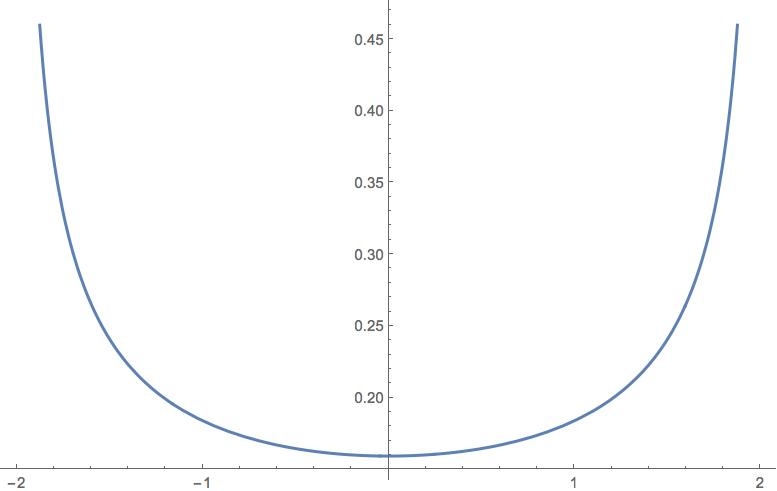
\includegraphics[width=.6\textwidth]{img/arcsine.png}
	\caption{The arcsine density.}
	\label{fig:arcsine}
\end{figure}

\begin{exercise}[Free Poisson Theorem]
Let $\alpha>0, \lambda>1$, and consider the Bernoulli density
\begin{align*}
    \mu_N=(1-\lambda/N)\delta_0+\lambda/N\delta_\alpha
\end{align*}
supported by $0$ and $\alpha$.
Classically, 
\begin{equation*}
    \mu_N^{*N}\to \mathrm{Poisson}(\lambda)
    \textnormal{\ on $\{0,\alpha,2 \alpha,\ldots\}$}
    ,\qquad N\to\infty.
\end{equation*}

In the free situation, by computing the R-transform, multiplying it by $N$, 
and then inverting, show that $\mu_N^{\boxplus N}$ 
converges to the density $\frac{1}{2\pi\alpha t}\sqrt{4\lambda\alpha^2-(t-\alpha(1+\lambda))^2}$, 
which is the Marchenko--Pastur distribution (\Cref{ssub:marchenko_pastur_law})
under a change of parameters. 
If $\lambda\le1$, then the limiting distribution is different. Namely, it has an atom of size $1- \lambda$ at $0$,
and the rest of the mass $\lambda$ is distributed according to the same Marchenko--Pastur law.
\end{exercise}

\begin{exercise}[{Cauchy Density}]
Show that for the Cauchy density $C=\frac{1}{\pi(1+x^2)}$ on $\mathbb{R}$, 
\begin{align*}
    \mu*C=\mu\boxplus C,
\end{align*}
i.e., the free convolution with the Cauchy density is the same as the classical convolution.
See \cite[Exercise 5.3.41]{AndersonGuionnetZeitouniBook} for more hints.
\end{exercise}

% subsection examples_of_free_convolutions (end)

\subsection{Notes and references} % (fold)
\label{sub:notes_Free}

Free Probability was invented by Voiculescu in the 1980s
to study operator algebras
(e.g., \cite{Voiculescu_Free_book} gives an early introduction).
In particular, the word ``free'' comes from the free groups.
Studying operator algebras associated with the free groups 
was one of the motivations for developing Free Probability.
In our discussions we mainly follow Chapter 5 of \cite{AndersonGuionnetZeitouniBook},
and also lecture notes \cite{Novak2012FreeLectures} which provide a lot of combinatorial
insights into Free Probability.

% subsection notes (end)

% section elements_of_free_probability (end)

\section{Gaussian Unitary Ensemble and its asymptotic behavior} % (fold)
\label{sec:gaussian_unitary_ensemble}

\subsection{Definition and basic properties} % (fold)
\label{sub:definition_and_basic_properties}

Recall that by $\mathcal H_N$ we denote the set of $N \times N$ Hermitian matrices over $\mathbb{C}$. 

\begin{definition}
  The law of the Gaussian Unitary Ensemble (GUE) is 
  a probability distribution on $\mathcal H_N$, and the law of 
  a random matrix $A=(a_{ij})_{i,j=1}^N\in\mathcal H_N$ is described as follows:
  \begin{itemize}
    \item $a_{ii} \sim \mathcal{N}(0,1)$ for each $i$.
    \item $a_{ij}=\overline{a}_{ji}\sim \mathcal{N}(0,1/2)+ \sqrt{-1}\, \mathcal{N}(0,1/2)$ for $i<j$.
  \end{itemize}
  All real normal random variables involved above are assumed to be independent.
  Note that $\EE a_{ij}=0$ for all $i,j$.
\end{definition}

Now fix any (nonrandom) $A\in \mathcal H_N$. Then we can write
\begin{equation*}
  \mathrm{tr}(A^2)=\mathrm{tr}(AA)=\sum_{i=1}^N a_{ii}^2+\sum_{i\neq j} a_{ij}a_{ji}=\sum_{i=1}^N a_{ii}^2+2\sum_{i<j} |a_{ij}|^2.
\end{equation*}
Identify $\mathcal H_N$ with $\mathbb{R}^{N^2}$ with the standard Lebesgue measure
which in the matrix coordinates can be written as
\begin{align*}
  dA = \prod_i d a_{ii} \prod_{i<j} da_{ij}^{\Re} da_{ij}^\Im.
\end{align*}
Here the superscripts $\Re$ and $\Im$ refer to the real and imaginary parts.

The GUE distribution $\mu$ on $\mathcal H_N$
has probability density (with respect to the above Lebesgue measure)
\begin{align*}
  d\mu(A) &=\frac{1}{Z_N}e^{-\sum_{i}a_{ii}^2/2}
  e^{-\sum_{i<j}(a_{ij}^{\Re})^2-\sum_{i<j}(a_{ij}^{\Im})^2} dA \\
  &= \frac{1}{Z_N}e^{-\frac{1}{2}(\sum_i a_{ii}^2+2\sum_{i<j}|a_{ij}|^2)} dA\\
  &= \frac{1}{Z_N} e^{-\frac{1}{2} \mathrm{tr}(A^2)} dA,
\end{align*}
where $Z_N=(\sqrt{\pi})^{N^2} (\sqrt{2})^N$ is the normalization constant (its value
follows from the normalization of the Gaussian distribution).

This computation shows that the GUE density
is \emph{unitary invariant}. That is, if $A$ is a random matrix with GUE distribution 
and $U\in U(N)$ is a fixed unitary matrix, 
then $U A U^{-1}\stackrel{\mathcal D}{=}A$ (equality in distribution).

% subsection definition_and_basic_properties (end)

\subsection{Joint eigenvalue density} % (fold)
\label{sub:joint_eigenvalue_density}

Let $A\in\mathcal H_N$ have the GUE distribution.
Denote its 
eigenvalues (which are necessarily real) by $\lambda_1\ge\cdots\ge\lambda_N$.

\begin{exercise}
	Show that under the GUE distribution the eigenvalues of the matrix
	are almost surely pairwise distinct.
\end{exercise}

We will now derive the joint density of eigenvalues of the GUE random matrix:

\begin{theorem}\label{thm:eigenvalue_density}
  Let $A=A_N\in\mathcal H_N$ have the GUE distribution. 
  Then the joint density of the eigenvalues of $A$ 
  with respect to the Lebesgue measure on $\mathbb{R}^{N}$ is given by
  \begin{equation*}
    C_N \prod_{i<j} |\lambda_i-\lambda_j|^2 \prod_{i=1}^N e^{-\lambda_i^2/2}.
  \end{equation*}
\end{theorem}
We will not compute the value of the normalization
constant $C_N$ right now, but later in \Cref{sub:determinantal_structure_of_the_gue} we will see that it is equal to 
$\dfrac{(2\pi)^{-N/2}}{0! 1!\cdots (N-1)!N!}$ (see also \Cref{rmk:ordering} below
on a slight ambiguity in the value of this normalization constant).
\begin{proof}
  We will in fact prove a more general result.
  Namely,
  let $f$ be a function on the space $\mathcal H_N$ of 
  Hermitian $N\times N$ matrices 
  which is unitary invariant, 
  i.e. $f(U A U^*)=f(A)$ for any fixed unitary matrix $U$. 
  (This implies that $f$ depends only on the eigenvalues $\lambda_1,\ldots, \lambda_N$ of $A$, and 
  moreover, in a symmetric way.) We will show that
  \begin{equation}\label{radial_part_Lebesgue_unitary}
    \int_{\mathcal H_N}f(A) dA=\mathrm{const}_N\int_{\mathbb{R}^N} f(\lambda_1,\ldots, \lambda_N) 
    \prod_{i<j} |\lambda_i-\lambda_j|^2 ~ d\lambda_1\cdots d\lambda_N,
  \end{equation}
  where both integrals are with respect to the corresponding Lebesgue measures. 
  In other words, we aim to find
  the Jacobian of the transformation mapping from $A$ to the set of its eigenvalues.

  \begin{example}
	As an example, consider the change of coordinates in $\mathbb{R}^2$ from Cartesian to polar: $(x,y)\to (r,\theta)$. If $f(x,y)$ is independent of $\theta$, i.e. it is radially symmetric, then
	\begin{equation*}
	\iint_{\mathbb{R}^2} f(x,y) ~ dxdy =2\pi \int_0^\infty f(r) r dr.
	\end{equation*}
	The factor $r$ comes from the Jacobian, and so 
	$2\pi r=\mathrm{const}\cdot r$ is the \emph{radial part} of the 
	Lebesgue measure on $\mathbb{R}^2$. 
	What we are about to do now is a generalization of this procedure.
	That is, we will find the radial part of the Lebesgue measure on the 
	space of $N\times N$ Hermitian matrices.
  \end{example}

  Continuing with the proof,
  view $\mathcal H_N$ as a space with an action of the unitary group $U(N)$ by conjugations: $A\mapsto UAU^*$. 
  A typical matrix\footnote{That is, almost every matrix with 
  respect to the GUE (or, equivalently, the Lebesgue) measure on $\mathcal H_N$.}
  $A\in \mathcal H_N$ can be written as $U \Lambda U^*$, where $\Lambda$ is the diagonal matrix of eigenvalues of $A$. 
  This gives rise to a change of variables 
  \begin{equation*}
    A \leftrightarrow (\vec{\lambda}, \dot{U}),
  \end{equation*}
  where $\vec{\lambda}$ is the vector of eigenvalues and $\dot{U}=U \mod T$, 
  where $T$ is the torus of diagonal matrices 
  which stabilize $\vec{\lambda}$. The matrix $\dot{U}$ represents the rotation to the eigenbasis of $A$.
  
  The Jacobian we aim to compute is $dA=(?) d\vec{\lambda} d \dot{U}$, where $d\dot{U}$ is Haar measure. 
  We note that the Jacobian must be independent of $U$ since the Lebesgue measure is rotationally invariant.
  
  Let us write $U=1+X$ where $X$ is ``small''. In other words,
  we are applying a Lie algebraic perspective. Since $U$ is unitary, the 
  matrix $X$ must be skew-Hermitian: $X+X^*=0$.
  This leaves $N^{2}$ real parameters in $X$ (which corresponds to the well-known
  fact that $U(N)$ is $N^{2}$-dimensional over $\mathbb{R}$).
  Then $U^*=U^{-1}=1-X+\textnormal{smaller order terms}$. 
  Since $A=U\Lambda U^*$, we can write
  \begin{equation*}
    A+dA=(1+X)(\Lambda+d\Lambda)(1-X)=\Lambda+d\Lambda+X\Lambda-\Lambda X+\textnormal{smaller order terms}.
  \end{equation*}
  Hence small changes in diagonal terms in $A$
  are 
  \begin{equation*}
  	d a_{ii} = d\lambda_i,
  \end{equation*}
  while small changes in the off-diagonal terms have the form (here $j< k$)
  \begin{align*}
    d a_{jk} = x_{jk}\lambda_k-\lambda_j x_{jk}=(\lambda_k-\lambda_j)x_{jk}.
  \end{align*}
  Since both $da_{jk}$ and $x_{jk}$ are complex, the contribution 
  $(\lambda_k-\lambda_j)$ affects both 
  $da_{jk}^{\Re}$ and $da_{jk}^{\Im}$, so overall we see that the 
  the Jacobian is $\prod_{j<k} |\lambda_j-\lambda_k|^2$.
  
  The theorem then follows from \eqref{radial_part_Lebesgue_unitary}
  by setting $f(A)=e^{-\frac{1}{2} \mathrm{tr}(A^2)}$.
\end{proof}

% subsection joint_eigenvalue_density (end)

\subsection{Other random matrix ensembles with explicit eigenvalue density} % (fold)
\label{sub:other_gaussian_ensembles}

The eigenvalue density result of \Cref{thm:eigenvalue_density} opens a way to generalize the Gaussian
Unitary Ensemble in several directions.
We can express the joint eigenvalue density of a GUE using the Vandermonde determinant
\begin{equation*}
  V(\lambda)=\prod_{i<j} |\lambda_i-\lambda_j|.
\end{equation*}
\begin{exercise}
  Show that $V(\lambda)=\pm \Det_{i,j=1}^{N} \lambda_i^{j-1}.$
\end{exercise}
The density of eigenvalues of \Cref{thm:eigenvalue_density}
is 
\begin{equation*}
  C_N^{GUE} V(\lambda)^2 \prod_{i=1}^N e^{-\frac{1}{2}\lambda_i^2}.
\end{equation*}

\subsubsection{Beta ensembles} % (fold)
\label{ssub:beta_ensembles}

Certain other Gaussian random matrix ensembles 
defined similarly to the GUE
have eigenvalue densities also involving $V(\lambda)$.

Recall that a real symmetric matrix $A$ has 
Gaussian Orthogonal Ensemble (GOE) distribution 
if $a_{ii}\sim \mathcal{N}(0,2)$ and $a_{ij}=a_{ji}\sim \mathcal{N}(0,1)$ for $i<j$. Then the GOE eigenvalue density is 
\begin{equation*}
  C_N^{GOE} |V(\lambda)|\prod_{i=1}^N e^{-\lambda_i^2/4}
\end{equation*}
with respect to the Lebesgue measure on $\mathbb{R}^{N}$.

The powers of $V(\lambda)$ can be generalized, leading to Gaussian $\beta$ Ensembles (G$\beta$E), 
with eigenvalue density (with respect to Lebesgue measure) given by
\begin{equation}\label{beta_ensemble}
  C_N^{\beta} |V(\lambda)|^{\beta} \prod_{i=1}^N e^{-(\lambda_i^2/4)\beta}.
\end{equation}
For certain special values of $\beta$ the above density
is a probability density of eigenvalues of random matrices:
\begin{equation*}
	\begin{tabular}{ccc}
	  $\beta=1$ & GOE & $\mathbb{R}$ \\
	  $\beta=2$ & GUE & $\mathbb{C}$ \\
	  $\beta=4$ & G Symplectic E (GSE) & $\mathbb{H}$
	\end{tabular}
\end{equation*}
(We will not define the GSE here --- see, for example, \cite{mehta2004random}.)
No other values of $\beta$ correspond to similar invariant random matrix ensembles. 
However, there are still ways to study general G$\beta$E. In fact, the spectral distributions
of these ensembles still converge to the Wigner semicircle law (but the local limiting distributions
are substantially different).

One way to treat the Gaussian $\beta$ ensembles is to introduce a completely different
random matrix model for the spectral distribution \eqref{beta_ensemble}.
This was first observed in 
\cite{dumitriu2002matrix} by applying the standard tridiagonalization procedure from
linear algebra to Gaussian random matrices, and reading off the corresponding distributions.
This tridiagonal matrix ensemble for G$\beta$E looks as follows. 
Let $\chi_t$ be a $\chi$ random variable of parameter $t$, that is, with density 
\begin{equation*}
  \frac{2^{1-t/2} x^{t-1} e^{-x^2/2}}{\Gamma(t/2)}
\end{equation*}
on the real line.
Let $y_i \sim \chi_{i\beta}$, $\xi_i\sim \mathcal{N}(0,1)$ be independent random variables. Then the tridiagonal ensemble 
\begin{equation*}
  A_N^\beta=\begin{bmatrix}
    \sqrt{\frac{2}{\beta}}\xi_1 & y_{N-1}/\sqrt{\beta} &  \dots & 0 \\
    y_{N-1}/\sqrt{\beta} & \sqrt{\frac{2}{\beta}}\xi_2 & \ddots &  \vdots \\
    \vdots & \ddots & \ddots &   y_{1}/\sqrt{\beta} \\
    0 & \dots & y_{1}/\sqrt{\beta} & \sqrt{\frac{2}{\beta}} \xi_N 
  \end{bmatrix}
\end{equation*}
has the eigenvalue density G$\beta$E.

One can view the above matrix $A_N^\beta$ as a linear operator, in this case it will be a 
\emph{random difference operator}.
As $N\to \infty$ it converges to a random differential operator. This analysis is performed in,
e.g., \cite{RamirezRiderVirag2006RandomAiry}.

\begin{remark}
  Eigenvalue densities are also accessible for Gaussian random matrices without Hermitian or real symmetry. 
  That is, if the elements of a random matrix
  $a_{ij}\sim \mathcal{N}(0,1)$ are i.i.d. for all $i,j$, then the spectrum
  of this matrix (which is complex)
  is the so-called Ginibre ensemble. The limiting spectral distribution
  in this case is uniform on the unit disc in the complex plane. This result
  is known under the name \emph{Girko's Circular Law}.
\end{remark}

% subsubsection beta_ensembles (end)

\subsubsection{Circular ensembles} % (fold)
\label{ssub:circular_ensembles}

Another example is the Circular Dyson's ensemble (CUE) of random matrices.
Consider the Haar measure $\mu$ on the compact group of unitary matrices $U(N)$. This measure is shift invariant, i.e.
\begin{equation*}
  \forall \mathcal{A}\subseteq U(N),\ \forall V\in U(N),\qquad \mu(V\mathcal{A})=\mu(\mathcal{A}V)=\mu(\mathcal{A}),
\end{equation*}
and is normalized so $\mu(U(N))=1$.

The eigenvalues of a random matrix $U_N\in U(N)$ lie on the unit circle, so they are of the form $e^{i\theta_k}, k=1,\ldots, N$. The joint density of the eigenvalues is 
\begin{equation*}
  C_N^{CUE} \prod_{k<j} |e^{i\theta_k}-e^{i\theta_j}|^2
\end{equation*}
with respect to the Lebesgue measure on the $N$-dimensional torus $\{|z|=1\}^N$. 
This ensemble does not have any edge behavior, so we will not consider it. 
The local (bulk) distribution in the CUE case is similar to that of the Gaussian Unitary Ensemble
with real eigenvalues.

It is also possible to define general $\beta$ CUE ensembles by changing the power of the Vandermonde determinant.


% subsubsection circular_ensembles (end)

\subsubsection{Invariant ensembles} % (fold)
\label{ssub:invariant_ensembles}

\note{log-gas interpretation of the eigenvalue density, and invariant ensembles --- to be filled in here}

% subsubsection invariant_ensembles (end)

% subsection other_gaussian_ensembles (end)

\lect{2/10/2016}

\subsection{Determinantal structure of the GUE} % (fold)
\label{sub:determinantal_structure_of_the_gue}
We now return to the GUE case, and investigate 
its joint eigenvalue density in more detail. 

\subsubsection{Correlation functions} % (fold)
\label{ssub:correlation_functions}

Recall that the GUE joint probability density 
with respect to the Lebesgue measure has the form
$C_N V(x)^2 \prod_{i=1}^{N} e^{-x_i^2/2}$,
where $V(x)$ is the Vandermonde determinant.
\begin{remark}\label{rmk:ordering}
	Note that the joint GUE eigenvalue density is invariant under permutations
	of the $x_i$'s, which creates an ambiguity on which space one should consider the 
	density --- the whole $\mathbb{R}^{N}$ or the ordered cone 
	$\mathbb{W}^{N}:=\{x_1\ge \ldots\ge x_N\}\subset\mathbb{R}^{N}$?\footnote{The space
	$\mathbb{W}^{N}$ is sometimes also called the \emph{Weyl chamber}.} 
	The difference between these choices leads to an additional factor of $N!$ in the normalization
	constant $C_N$.
	Here we will adopt the first 
	convention, and will think of the argument in 
	the joint density as an element of $\mathbb{R}^{N}$.
\end{remark}
According to \Cref{thm:eigenvalue_density}
and with the understanding of
\Cref{rmk:ordering}, the joint probability density of eigenvalues
of the GUE matrix has the form
\begin{equation}\label{GUE_density}
	\tilde \rho_N(x_1,\ldots,x_N)=C_N \prod_{1\le i<j\le N}|x_i-x_j|^{2} \prod_{i=1}^{N} e^{-x_i^2/2},\qquad
	x=(x_1,\ldots,x_N)\in\mathbb{R}^{N}.
\end{equation}

\begin{definition}
  The function $\rho_k:\mathbb{W}^k\to \mathbb{R}$, 
  where $\rho_k(y_1,\dots, y_k)$ is the probability density (with respect to the Lebesgue measure on 
  the space $\mathbb{W}^{k}$ of $k$-point configurations)
  to find eigenvalues close to $y_1,\cdots, y_k$, 
  is called the $k$th \emph{correlation function}.

  Note that the argument of the correlation function $\rho_k$ 
  is a point configuration and not an element of $\mathbb{R}^{k}$.
  The arguments in the correlation function must be distinct, otherwise
  it vanishes by agreement.
\end{definition}
\begin{example}
  The first correlation function
  $\rho_1(y_1)$ is called the \emph{density function}; it may be used to get the semicircle law.
\end{example}
\begin{remark}
	The correlation function $\rho_k$
	is not necessarily a probability density function, because it does not necessarily integrate to 1.
	For example, 
	$\int_{a}^{b}\rho_{1}(y_1)dy_1$ is the expected number of eigenvalues
	in the segment $[a,b]$.
\end{remark}


We can compute $\rho_k(y_1,\cdots, y_k)$ as follows:
\begin{equation*}
  \rho_k(y_1,\cdots, y_k)=\int_{\mathbb{R}^{N-k}} \frac{N!}{(N-k)!} 
  \,\tilde \rho_N(y_1,\cdots, y_k, x_{k+1}, \cdots, x_N) dx_{k+1}\cdots dx_N.
\end{equation*}
In particular, $\rho_N(x_1,\ldots,x_N)=N!\, \tilde \rho_N(x_1,\ldots,x_N)$
for $(x_1,\ldots,x_N)\in\mathbb{W}^{N}$, which makes sense
because $(x_1,\ldots,x_N)$ in the left-hand side is a point configuration, and 
to get $\rho_N(x_1,\ldots,x_N)$ one should sum the values of $\tilde \rho_N$
over all permutations.

We will now work towards showing that the correlation functions 
$\rho_k$ are given by $k\times k$ determinants of a certain form.

% subsubsection correlation_functions (end)

\subsubsection{Determinantal point processes and biorthogonal ensembles} % (fold)
\label{ssub:determinantal_point_processes}

By a \emph{point process} (say, on $\mathbb{R}$) we mean a probability measure on the 
space of point configurations on $\mathbb{R}$. In this
way the eigenvalues of the GUE random matrix form a point process on $\mathbb{R}$
(which has $N$ points almost surely).

\begin{definition}\label{def:}
  If there exists a function $K(x,y)$ such that 
  for any $k$ and any pairwise distinct $y_1,\ldots,y_k$ one has
  $\rho_k(y_1,\ldots,y_k)=\Det_{i,j=1}^{k}K(y_i,y_j)$,
  then the point process is called \emph{determinantal}.
\end{definition}

We will now obtain a formal statement showing that certain probability distributions
on $N$-point configurations are determinantal, and will compute the corresponding
correlation kernels. 
Let $(\mathfrak{X},\mu)$ be a ``sufficiently nice'' space with a probability measure.
Define a distribution on the space of $N$-point configurations on $\mathfrak{X}$:
\begin{equation}\label{biorthogonal_ensemble}
  P(dx_1\cdots dx_N)=C_N \Det_{i,j=1}^{N}\phi_i(x_j)\cdot \Det_{i,j=1}^{N}\psi_i(x_j)\cdot \mu(dx_1)\cdots\mu(dx_N),
\end{equation}
where $\phi_1,\ldots,\phi_N$ and $\psi_1,\ldots,\psi_N$ are fixed functions on $\mathfrak{X}$
and
$C_N$ is the normalization constant.
\begin{example}
	For example, if $\mathfrak{X}=\mathbb{R}$,
	$\mu$ is the standard normal distribution, and 
	$\phi_i(x)=\psi_i(x)=x^{i-1}$, 
	then the measure \eqref{biorthogonal_ensemble} corresponds to the GUE spectrum.
\end{example}

We will now proceed to the computation of the correlation kernel of the 
point process \eqref{biorthogonal_ensemble}.

\textbf{Step 1.}
Set $G_{ij}=\int_{\mathfrak{X}} \phi_i(x)\psi_j(x) \mu(dx)$. The matrix $G=[G_{ij}]_{i,j=1}^N$ is 
sometimes called the ``Gram matrix''. Then 
\begin{align*}
  \frac{1}{C_N} &= \idotsint \Det_{i,j=1}^{N}\phi_i(x_j) \Det_{i,j=1}^{N}\psi_i(x_j) \mu(\vec{dx}) \\
  &= \sum_{\sigma, \tau\in S_N} (-1)^{\sigma} (-1)^{\tau} \prod_{i=1}^N \int_{\mathfrak{X}} \phi_{\sigma(i)}(x_i) \psi_{\tau(i)}(x_i) \mu(dx_i) \\
  &= \sum_{\sigma, \tau\in S_N} (-1)^{\sigma} (-1)^{\tau} \prod_{i=1}^N G_{\sigma(i)\tau(i)} \\
  &= N! \det[G].
\end{align*}
Above we have expanded the determinants
as summations over the symmetric group $S_N$,
and rewrote the result as a new determinant.
The above computation implies that $G$ is invertible. 

\textbf{Step 2.} Let us now compute the correlation functions
\begin{equation*}
  \rho_k(x_1,\cdots, x_k)=\frac{N!}{(N-k)!}
  \idotsint_{\mathfrak{X}^{N-k}} 
  \Det_{i,j=1}^{N}\phi_i(x_j)\Det_{i,j=1}^{N}\psi_i(x_j) \frac{\mu(dx_{k+1})\ldots
  \mu(dx_N)}{N!\det[G]}.
\end{equation*}
Since $G$ is invertible, there exist $N\times N$
matrices $A, B$ such that $AGB^T=1$.\footnote{Note that
their choice is not unique,
which can be helpful in some applications.} 
Define $\Phi_k=\sum_{l=1}^{N} A_{kl}\phi_l$ and $\Psi_k=\sum_{l=1}^{N} B_{kl}\psi_l$. Then clearly
\begin{equation}\label{biorthogonality}
  \int_{\mathfrak{X}}\Phi_k(x)\Psi_l(x)\mu(dx)=\delta_{kl},
\end{equation}
that is, the functions $\Phi_k$ and $\Psi_l$ form a \emph{biorthogonal family}.
For this reason the probability distribution \eqref{biorthogonal_ensemble}
is sometimes referred to as the \emph{biorthogonal ensemble}.

Using these biorthogonal functions, the measure \eqref{biorthogonal_ensemble} takes the form
\begin{equation*}
  P(dx_1,\ldots,dx_N)=\frac{1}{N!} \Det_{i,j=1}^{N}\Phi_i(x_j)\cdot \Det_{i,j=1}^{N}\Psi_i(x_j)\cdot \mu(dx_1)\ldots\mu(dx_N).
\end{equation*}

\textbf{Step 3.}
Thus, the correlation functions have the form
\begin{equation*}
  \rho_n(x_1,\cdots, x_n)=\frac{1}{(N-n)!}\idotsint_{\mathfrak{X}^{N-n}} 
  \sum_{\sigma, \tau\in S_N} (-1)^{\sigma}(-1)^{\tau} 
  \bigg(\prod_{i=1}^N \Phi_{\sigma(i)}(x_i)\Psi_{\tau(i)}(x_i)\bigg)
  \mu(dx_{k+1})\ldots\mu(dx_N).
\end{equation*}
By the biorthogonality, nonzero terms in the above sum must have $\sigma(k)=\tau(k)$, $k=n+1,\cdots, N$, so
\begin{equation}
  \rho_n(x_{n+1},\cdots, x_N) = \frac{1}{(N-n)!} \sum_{1\leq j_1\leq\cdots\leq j_n\leq N} \det[\Phi_{x_1,\cdots, x_n}^{j_1,\cdots, j_n}] \det[\Psi_{x_1,\cdots, x_n}^{j_1,\cdots, j_n}] 
  = \Det_{i,j=1}^{n}\bigg[\sum_{k=1}^N \Phi_k(x_i) \Psi_k(x_j)\bigg].
  \label{Final_computation_of_corr_kernel}
\end{equation}
We now explain these two equalities and the notation. 
By $\Phi_{x_1,\cdots, x_n}^{j_1,\cdots, j_n}$ 
we mean the $n$ by $n$ matrix consisting of the 
intersection of the first $n$ rows of $[\Phi_j(x_i)]$ 
and the $n$ columns corresponding to $j_1,\cdots, j_n$,
and similarly for $\Psi_{x_1,\cdots, x_n}^{j_1,\cdots, j_n}$.
The first equality follows by the biorthogonality \eqref{biorthogonality}, and 
to obtain the second equality we have used the \emph{Cauchy-Binet formula} from the next proposition.

\begin{proposition}[Cauchy-Binet formula]
	Let $A$ be an $m\times n$ matrix 
	and $B$ an $n\times m$ matrix. 
	If $J\subseteq \{1,\cdots, n\}$ has size $m$, 
	let $A_J$ be the $m\times m$ submatrix of $A$ 
	with columns from $J$, and let $B_J$ be the $m\times m$ submatrix of $B$ with rows from $J$. Then
	\begin{equation*}
	  \det(AB)=\sum_{J\subseteq \{1,\cdots, n\}\colon|J|=m} \det(A_J) \det(B_J).
	\end{equation*}
\end{proposition}

\textbf{Step 4.}
The computation \eqref{Final_computation_of_corr_kernel}
implies that the point process
\eqref{biorthogonal_ensemble} is determinantal with the correlation kernel
$K(x,y)=\sum \Phi_k(x) \Psi_k(y)$. As written, it depends on the choice of $A$ and $B$,
but one can rewrite it in the form
\begin{equation}\label{biorthogonal_ensemble_kernel}
	K(x,y)=\sum_{i,j=1}^N [G^{-1}]_{ji}\, \phi_i(x) \psi_j(y)
	=\sum_{i,j=1}^N [G^{{}-{}\textnormal{transpose}}]_{ij}\, \phi_i(x) \psi_j(y),
\end{equation}
so the kernel is in fact independent of the choice of $A$ and $B$.

\begin{remark}\label{rmk:reference_measure}
	In this general setting, the correlation functions 
	$\rho_k(y_1,\ldots,y_k)$ are defined with respect to the \emph{reference measure}
	$\mu$
	on $\mathfrak{X}$.
	That is,
	$\rho_k(y_1,\ldots,y_k)\mu(dy_1)\ldots\mu(dy_k)$ is the infinitesimal probability
	to find particles from the point process around the locations
	$y_1,\ldots,y_k$.
	Therefore, the kernel $K(x,y)$ is also defined with respect to the same reference measure.
	Later, when talking about scaling limits of correlation kernels, 
	an appropriate object would be 
	\begin{equation}\label{reference_measure_invariant_form}
		K(x,y)\sqrt{\mu(dx)\mu(dy)},
	\end{equation}
	or, in other words, an integral operator in $L^2(\mu)$.
\end{remark}

% subsubsection determinantal_point_processes (end)

\subsubsection{Correlation kernel for the GUE} % (fold)
\label{ssub:correlation_kernel_for_the_gue}

Applying the computation of \Cref{ssub:determinantal_point_processes}
to the GUE setting, we let 
$\mu(dx)=\frac{1}{\sqrt{2\pi}}e^{-x^2/2}$ be the standard $\mathcal{N}(0,1)$ distribution,
and $\phi_i(x)=\psi_i(x)=x^{i-1}$ be the power functions. 
To get a formula for the correlation
kernel of the GUE, let us orthogonalize the powers $x^{i-1}$ with respect to the weight $e^{-x^2/2}$. We have
\begin{equation}\label{GUE_via_Hermite}
  P_{GUE}(dx_1,\cdots, dx_N)=
  \frac{1}{N!}
  \Big(\Det_{i,j=1}^{N}H_{i-1}(x_j)\Big)^2 \mu(dx_1)\cdots\mu(dx_N),
\end{equation}
where the $H_i$'s are orthogonal polynomials called the \emph{Hermite polynomials}:
\begin{equation*}
  \int H_k(x) H_l(x) \mu(dx)=\delta_{kl},\qquad k,l=0,\ldots,N-1.
\end{equation*}

We have thus established the following result:
\begin{theorem}\label{thm:GUE_kernel}
	The random point process \eqref{GUE_density}, \eqref{GUE_via_Hermite}
	corresponding to the GUE eigenvalues is determinantal, with the correlation
	kernel (with respect to the standard normal
	reference measure, cf. \Cref{rmk:reference_measure})
	\begin{equation}
		K_N(x,y)=\sum_{j=0}^{N-1}H_j(x)H_j(y).
	\end{equation}
\end{theorem}

The asymptotics of the kernel $K_N$ determine the asymptotics of the GUE eigenvalues.

% subsubsection correlation_kernel_for_the_gue (end)

% subsection determinantal_structure_of_the_gue (end)

{\ }\\\lect{2/17/2016}

\subsection{Non-rigorous asymptotics via spectral projections} % (fold)
\label{sub:non_rigorous_asymptotics_using_operator_approach}

\note{put all stuff about Hermite polynomials in \Cref{sub:hermite_polynomials}, and reference it here}

% subsection non_rigorous_asymptotics_using_operator_approach (end)

{\ }\\\lect{3/14/2016}

\subsection{Hermite polynomials} % (fold)
\label{sub:hermite_polynomials}

% subsection hermite_polynomials (end)

{\ }\\\lect{3/16/2016}

\subsection{Rigorous asymptotics via contour integrals (Plancherel--Rotach asymptotics)} % (fold)
\label{sub:rigorous_asymptotics_via_contour_integrals}

\cite{Plancherel_Rotach_original}

% subsection rigorous_asymptotics_via_contour_integrals (end)

\subsection{Edge asymptotics} % (fold)
\label{sub:edge_asymptotics}

% subsection edge_asymptotics_and_the_tracy_widom_distribution (end)

\subsection{Inclusion/exclusion and Fredholm determinants} % (fold)
\label{sub:inclusion_exclusion_and_fredholm_determinants}

% subsection inclusion_exclusion_and_fredholm_determinants (end)

\subsection{Tracy--Widom distribution} % (fold)
\label{sub:tracy_widom_distribution}

\cite{TW_Airy_Painleve_2002}

% subsection tracy_widom_distribution (end)


\subsection{Notes and references} % (fold)
\label{sub:notes_GUE}

The material in \Cref{sec:gaussian_unitary_ensemble} represents a classical 
chapter in random matrix theory. 
The Gaussian Unitary Ensemble is a random matrix ensemble for which all the computations
can be carried out explicitly. 
\Cref{sub:non_rigorous_asymptotics_using_operator_approach}
closely follows the book \cite{TaoRMbook}.

The proof that the variational problem for the limiting spectral distribution
reduces to the Euler--Lagrange equations
(for which a naive argument was given in \Cref{ssub:invariant_ensembles})
may be deduced from \cite{saff2013logarithmic}, see also \cite{Forrester-LogGas}.

Generalities and details on determinantal point processes can be found in the 
surveys \cite{Soshnikov2000}, 
\cite{peres2006determinantal},
\cite{Borodin2009}.

The asymptotic results for the GUE presented here
are believed to be \emph{universal} --- that is,
they should not depend on the concrete structure of the 
ensemble and hold in much greater generality. 
Getting such universal results for random matrices 
is an important ongoing program which is successful so far in 
the bulk case (with getting the sine kernel).
See, e.g.,
\cite{Johansson2001Universality}, \cite{tao2011univ},
\cite{TaoVu2012Survey}, \cite{erdHos2011universality}.
Addressing some universality results is the next general goal of the course, for which we 
will need certain Markov processes on random matrices and on their spectra.

% subsection notes_GUE (end)

% section gaussian_unitary_ensemble (end)





\bibliography{bib}
\bibliographystyle{amsalpha}

\end{document}